\documentclass[11pt,fleqn, openany]{book} % Default font size and left-justified equations

%%%%%%%%%%%%%%%%%%%%%%%%%%%%%%%%%%%%%%%%%
% The Legrand Orange Book
% Structural Definitions File
% Version 2.1 (26/09/2018)
%
% Original author:
% Mathias Legrand (legrand.mathias@gmail.com) with modifications by:
% Vel (vel@latextemplates.com)
% 
% This file was downloaded from:
% http://www.LaTeXTemplates.com
%
% License:
% CC BY-NC-SA 3.0 (http://creativecommons.org/licenses/by-nc-sa/3.0/)
%
%%%%%%%%%%%%%%%%%%%%%%%%%%%%%%%%%%%%%%%%%

%----------------------------------------------------------------------------------------
%	VARIOUS REQUIRED PACKAGES AND CONFIGURATIONS
%----------------------------------------------------------------------------------------

\usepackage[table]{xcolor}

\usepackage{graphicx}
\usepackage{tabularx} % Required for including pictures
\usepackage{pgf,tikz,tkz-tab,eurosym,yhmath, stmaryrd}
\usepackage{pgfplots}
\usepackage{mathrsfs}
\usetikzlibrary{patterns}
\usetikzlibrary{trees}
\graphicspath{{../../Pictures/}}
\usepackage{multicol} 


\usepackage[english]{babel} % English language/hyphenation
\usepackage{icomma}
\usepackage{enumitem} % Customize lists
\setlist{nolistsep, nosep, nolistsep} % Reduce spacing between bullet points and numbered lists

\usepackage{booktabs} % Required for nicer horizontal rules in tables

 % Required for specifying colors by name


\definecolor{ocre}{RGB}{243,102,25} % Define the orange color used for highlighting throughout the book

\usepackage{listings}

\definecolor{codegreen}{rgb}{0,0.6,0}
\definecolor{codegray}{rgb}{0.5,0.5,0.5}
\definecolor{codepurple}{rgb}{0.58,0,0.82}
\definecolor{backcolour}{rgb}{0.95,0.95,0.92}

\lstdefinestyle{mystyle}{
    backgroundcolor=\color{backcolour},   
    commentstyle=\color{codegreen},
    keywordstyle=\color{magenta},
    numberstyle=\tiny\color{codegray},
    stringstyle=\color{codepurple},
    basicstyle=\ttfamily\footnotesize,
    breakatwhitespace=false,         
    breaklines=true,                 
    captionpos=b,                    
    keepspaces=true,                 
    numbers=left,                    
    numbersep=5pt,                  
    showspaces=false,                
    showstringspaces=false,
    showtabs=false,                  
    tabsize=2
}

\lstset{style=mystyle}

%----------------------------------------------------------------------------------------
% Paramétrage XSIM
%----------------------------------------------------------------------------------------

\usepackage[no-files]{xsim}


\DeclareExerciseEnvironmentTemplate{myex}{%
    \textbf{%
      \hypertarget{ex:\ExerciseID}{\sffamily{\ensuremath{\blacktriangleright}} Exercice \GetExerciseProperty{counter} \GetExerciseProperty{subtitle} --}
      \hyperlink{sol:\ExerciseID}{Voir le corrigé}%
    }\par
}{\par\smallskip}

\DeclareExerciseEnvironmentTemplate{mysol}{%
    \textbf{%
      \hypertarget{sol:\ExerciseID}{\sffamily{\ensuremath{\blacktriangleright}} Correction \GetExerciseProperty{counter} --}
      \hyperlink{ex:\ExerciseID}{Voir l'énoncé}%
    }\par
}{\par\medskip}

\xsimsetup{
  exercise/template = myex ,
  solution/template = mysol 
}

%Collection exercices

\DeclareExerciseTagging{topic}

\xsimsetup{collect}

%----------------------------------------------------------------------------------------
% SYMBOLES
%----------------------------------------------------------------------------------------

\newcommand\imCMsym[4][\mathord]{%
  \DeclareFontFamily{U} {#2}{}
  \DeclareFontShape{U}{#2}{m}{n}{
    <-6> #25
    <6-7> #26
    <7-8> #27
    <8-9> #28
    <9-10> #29
    <10-12> #210
    <12-> #212}{}
  \DeclareSymbolFont{CM#2} {U} {#2}{m}{n}
  \DeclareMathSymbol{#4}{#1}{CM#2}{#3}
}
\newcommand\alsoimCMsym[4][\mathord]{\DeclareMathSymbol{#4}{#1}{CM#2}{#3}}

\imCMsym{cmmi}{124}{\CMjmath}

\newcommand{\Oij}{(O\,;\,\vec{\imath}\,,\, \vec{\CMjmath} )}
\newcommand{\Oijk}{(O\,;\,\vec{\imath}\,,\, \vec{\CMjmath}\,,\,\vec{k})}

\newcommand\e{\mathrm{e}}
\newcommand\R{\mathbb{R}}
\newcommand\N{\mathbb{N}}


%----------------------------------------------------------------------------------------
%	MARGINS
%----------------------------------------------------------------------------------------

\usepackage{geometry} % Required for adjusting page dimensions and margins

\geometry{
	paper=a4paper, % Paper size, change to letterpaper for US letter size
	top=3cm, % Top margin
	bottom=3cm, % Bottom margin
	left=2cm, % Left margin
	right=2cm, % Right margin
	headheight=14pt, % Header height
	footskip=1.4cm, % Space from the bottom margin to the baseline of the footer
	headsep=10pt, % Space from the top margin to the baseline of the header
	%showframe, % Uncomment to show how the type block is set on the page
}

\setlength{\parindent}{0pt}
\parskip=5pt



%----------------------------------------------------------------------------------------
%	FONTS
%----------------------------------------------------------------------------------------

\usepackage{avant} % Use the Avantgarde font for headings
\usepackage{times} % Use the Times font for headings
\usepackage{mathptmx} % Use the Adobe Times Roman as the default text font together with math symbols from the Sym­bol, Chancery and Com­puter Modern fonts

%\usepackage{microtype} % Slightly tweak font spacing for aesthetics
%\usepackage[utf8]{inputenc} % Required for including letters with accents
\usepackage[T1]{fontenc} % Use 8-bit encoding that has 256 glyphs

%----------------------------------------------------------------------------------------
%	BIBLIOGRAPHY AND INDEX
%----------------------------------------------------------------------------------------

\usepackage[style=numeric,citestyle=numeric,sorting=nyt,sortcites=true,autopunct=true,babel=hyphen,hyperref=true,abbreviate=false,backref=true,backend=biber]{biblatex}
\addbibresource{bibliography.bib} % BibTeX bibliography file
\defbibheading{bibempty}{}

\usepackage{calc} % For simpler calculation - used for spacing the index letter headings correctly
\usepackage{makeidx} % Required to make an index
\makeindex % Tells LaTeX to create the files required for indexing

%----------------------------------------------------------------------------------------
%	MAIN TABLE OF CONTENTS
%----------------------------------------------------------------------------------------

\usepackage{titletoc} % Required for manipulating the table of contents

\contentsmargin{0cm} % Removes the default margin

% Part text styling (this is mostly taken care of in the PART HEADINGS section of this file)
\titlecontents{part}
	[0cm] % Left indentation
	{\addvspace{20pt}\bfseries} % Spacing and font options for parts
	{}
	{}
	{}

% Chapter text styling
\titlecontents{chapter}
	[1.25cm] % Left indentation
	{\addvspace{12pt}\large\sffamily\bfseries} % Spacing and font options for chapters
	{\color{ocre!60}\contentslabel[\Large\thecontentslabel]{1.25cm}\color{ocre}} % Formatting of numbered sections of this type
	{\color{ocre}} % Formatting of numberless sections of this type
	{\color{ocre!60}\normalsize\;\titlerule*[.5pc]{.}\;\thecontentspage} % Formatting of the filler to the right of the heading and the page number

% Section text styling
\titlecontents{section}
	[1.25cm] % Left indentation
	{\addvspace{3pt}\sffamily\bfseries} % Spacing and font options for sections
	{\contentslabel[\thecontentslabel]{1.25cm}} % Formatting of numbered sections of this type
	{} % Formatting of numberless sections of this type
	{\hfill\color{black}\thecontentspage} % Formatting of the filler to the right of the heading and the page number

% Subsection text styling
\titlecontents{subsection}
	[1.25cm] % Left indentation
	{\addvspace{1pt}\sffamily\small} % Spacing and font options for subsections
	{\contentslabel[\thecontentslabel]{1.25cm}} % Formatting of numbered sections of this type
	{} % Formatting of numberless sections of this type
	{\ \titlerule*[.5pc]{.}\;\thecontentspage} % Formatting of the filler to the right of the heading and the page number

% Figure text styling
\titlecontents{figure}
	[1.25cm] % Left indentation
	{\addvspace{1pt}\sffamily\small} % Spacing and font options for figures
	{\thecontentslabel\hspace*{1em}} % Formatting of numbered sections of this type
	{} % Formatting of numberless sections of this type
	{\ \titlerule*[.5pc]{.}\;\thecontentspage} % Formatting of the filler to the right of the heading and the page number

% Table text styling
\titlecontents{table}
	[1.25cm] % Left indentation
	{\addvspace{1pt}\sffamily\small} % Spacing and font options for tables
	{\thecontentslabel\hspace*{1em}} % Formatting of numbered sections of this type
	{} % Formatting of numberless sections of this type
	{\ \titlerule*[.5pc]{.}\;\thecontentspage} % Formatting of the filler to the right of the heading and the page number

%----------------------------------------------------------------------------------------
%	MINI TABLE OF CONTENTS IN PART HEADS
%----------------------------------------------------------------------------------------

% Chapter text styling
\titlecontents{lchapter}
	[0em] % Left indentation
	{\addvspace{15pt}\large\sffamily\bfseries} % Spacing and font options for chapters
	{\color{ocre}\contentslabel[\Large\thecontentslabel]{1.25cm}\color{ocre}} % Chapter number
	{}  
	{\color{ocre}\normalsize\sffamily\bfseries\;\titlerule*[.5pc]{.}\;\thecontentspage} % Page number

% Section text styling
\titlecontents{lsection}
	[0em] % Left indentation
	{\sffamily\small} % Spacing and font options for sections
	{\contentslabel[\thecontentslabel]{1.25cm}} % Section number
	{}
	{}

% Subsection text styling (note these aren't shown by default, display them by searchings this file for tocdepth and reading the commented text)
\titlecontents{lsubsection}
	[.5em] % Left indentation
	{\sffamily\footnotesize} % Spacing and font options for subsections
	{\contentslabel[\thecontentslabel]{1.25cm}}
	{}
	{}

%----------------------------------------------------------------------------------------
%	HEADERS AND FOOTERS
%----------------------------------------------------------------------------------------


\usepackage{fancyhdr} % Required for header and footer configuration

\pagestyle{fancy}
\renewcommand{\chaptermark}[1]{\markboth{\sffamily\normalsize\bfseries\ \thechapter.\ #1}{}} % Chapter text font settings
\renewcommand{\sectionmark}[1]{\markright{\sffamily\normalsize\thesection\hspace{5pt}#1}{}} % Section text font settings
\fancyhf{} \fancyhead[LE,RO]{\sffamily\normalsize\thepage} % Font setting for the page number in the header
\fancyhead[LO]{\rightmark} % Print the nearest section name on the left side of odd pages
\fancyhead[RE]{\leftmark} % Print the current chapter name on the right side of even pages

\fancyfoot[L]{Jason LAPEYRONNIE}
\fancyfoot[R]{\href{http://mathoutils.fr}{http://mathoutils.fr}} % Uncomment to include a footer

\renewcommand{\headrulewidth}{0.5pt} % Thickness of the rule under the header
\renewcommand{\footrulewidth}{0.5pt} % Thickness of the rule under the header

\fancypagestyle{plain}{% Style for when a plain pagestyle is specified
	\fancyhead{}\renewcommand{\headrulewidth}{0pt}%
}

% Removes the header from odd empty pages at the end of chapters
\makeatletter
\renewcommand{\cleardoublepage}{
\clearpage\ifodd\c@page\else
\hbox{}
\vspace*{\fill}
\thispagestyle{empty}
\newpage
\fi}

%----------------------------------------------------------------------------------------
%	THEOREM STYLES
%----------------------------------------------------------------------------------------

\usepackage{amsmath,amsfonts,amssymb,amsthm} % For math equations, theorems, symbols, etc

\newcommand{\intoo}[2]{\mathopen{]}#1\,;#2\mathclose{[}}
\newcommand{\ud}{\mathop{\mathrm{{}d}}\mathopen{}}
\newcommand{\intff}[2]{\mathopen{[}#1\,;#2\mathclose{]}}
\renewcommand{\qedsymbol}{$\blacksquare$}
\newtheorem{notation}{Notation}[section]

% Boxed/framed environments
\newtheoremstyle{ocrenumbox}% Theorem style name
{0pt}% Space above
{0pt}% Space below
{\normalfont}% Body font
{}% Indent amount
{\small\bf\sffamily\color{ocre}}% Theorem head font
{\;:\;}% Punctuation after theorem head
{0.25em}% Space after theorem head
{\small\sffamily\color{ocre}\thmname{#1}\nobreakspace\thmnumber{\@ifnotempty{#1}{}\@upn{#2}}% Theorem text (e.g. Theorem 2.1)
\thmnote{\nobreakspace\the\thm@notefont\sffamily\bfseries\color{black}---\nobreakspace#3}} % Optional theorem note

\newtheoremstyle{blacknumex}% Theorem style name
{5pt}% Space above
{10pt}% Space below
{\normalfont}% Body font
{} % Indent amount
{\small\bf\sffamily}% Theorem head font
{\;:\;}% Punctuation after theorem head
{0.25em}% Space after theorem head
{\small\sffamily{\tiny\ensuremath{\blacksquare}}\nobreakspace\thmname{#1}\nobreakspace\thmnumber{\@ifnotempty{#1}{}\@upn{#2}}% Theorem text (e.g. Theorem 2.1)
\thmnote{\nobreakspace\the\thm@notefont\sffamily\bfseries---\nobreakspace#3}}% Optional theorem note

\newtheoremstyle{blacknumexo}% Theorem style name
{15pt}% Space above
{10pt}% Space below
{\normalfont}% Body font
{} % Indent amount
{\small\bf\sffamily}% Theorem head font
{}% Punctuation after theorem head
{0.5em}% Space after theorem head
{\small\sffamily{\ensuremath{\blacktriangleright}}\nobreakspace\thmname{#1}\nobreakspace\thmnumber{\@ifnotempty{#1}{}\@upn{#2}}% Theorem text (e.g. Theorem 2.1)
\thmnote{\nobreakspace\the\thm@notefont\sffamily\bfseries---\nobreakspace#3} \\}% Optional theorem note



\newtheoremstyle{blacknumbox} % Theorem style name
{0pt}% Space above
{5pt}% Space below
{}% Body font
{}% Indent amount
{\large\bf\sffamily}% Theorem head font
{\;:\;}% Punctuation after theorem head
{0.25em}% Space after theorem head
{\small\sffamily\thmname{#1}\nobreakspace\thmnumber{\@ifnotempty{#1}{}\@upn{#2}}% Theorem text (e.g. Theorem 2.1)
\thmnote{\nobreakspace\the\thm@notefont\sffamily\bfseries---\nobreakspace#3}}% Optional theorem note

% Non-boxed/non-framed environments
\newtheoremstyle{ocrenum}% Theorem style name
{5pt}% Space above
{5pt}% Space below
{\normalfont}% Body font
{}% Indent amount
{\small\bf\sffamily\color{ocre}}% Theorem head font
{\;:\;}% Punctuation after theorem head
{0.25em}% Space after theorem head
{\small\sffamily\color{ocre}\thmname{#1}\nobreakspace\thmnumber{\@ifnotempty{#1}{}\@upn{#2}}% Theorem text (e.g. Theorem 2.1)
\thmnote{\nobreakspace\the\thm@notefont\sffamily\bfseries\color{black}---\nobreakspace#3}} % Optional theorem note
\makeatother

% Defines the theorem text style for each type of theorem to one of the three styles above
\newcounter{dummy} 
\newcounter{thm}
\newcounter{correction}
\newcounter{qst}
\theoremstyle{ocrenumbox}
\newtheorem{theoremeT}[dummy]{Théorème}
\newtheorem{exerciseT}{Propriété}
\newtheorem{principeT}{Principe}
\theoremstyle{blacknumex}
\newtheorem{exampleT}{Exemple}
\theoremstyle{blacknumexo}
\newtheorem{exo}[thm]{Exercice}
\newtheorem{corr}[correction]{Correction}
\newtheorem{quest}[qst]{Question}
\theoremstyle{blacknumbox}
\newtheorem{vocabulary}{Vocabulary}[section]
\newtheorem{definitionT}{Définition}
\newtheorem{corollaryT}[dummy]{Corollary}
\theoremstyle{ocrenum}
\newtheorem{proofT}[dummy]{Démonstration}


%----------------------------------------------------------------------------------------
%	DEFINITION OF COLORED BOXES
%----------------------------------------------------------------------------------------

\RequirePackage[framemethod=default]{mdframed} % Required for creating the theorem, definition, exercise and corollary boxes

% Theorem box
\newmdenv[skipabove=7pt,
skipbelow=7pt,
backgroundcolor=black!5,
linecolor=ocre,
innerleftmargin=5pt,
innerrightmargin=5pt,
innertopmargin=10pt,
leftmargin=0cm,
rightmargin=0cm,
innerbottommargin=5pt]{tBox}

%Proposition box	  
\newmdenv[skipabove=7pt,
skipbelow=7pt,
rightline=false,
leftline=true,
topline=false,
bottomline=false,
backgroundcolor=ocre!10,
linecolor=ocre,
innerleftmargin=5pt,
innerrightmargin=5pt,
innertopmargin=10pt,
innerbottommargin=3pt,
leftmargin=0cm,
rightmargin=0cm,
linewidth=4pt]{eBox}	

% Definition box
\newmdenv[skipabove=7pt,
backgroundcolor=ocre!4,
skipbelow=7pt,
rightline=false,
leftline=true,
topline=false,
bottomline=false,
linecolor=ocre,
innerleftmargin=5pt,
innerrightmargin=5pt,
innertopmargin=10pt,
leftmargin=0cm,
rightmargin=0cm,
linewidth=4pt,
innerbottommargin=5pt]{dBox}	

% Corollary box
\newmdenv[skipabove=7pt,
skipbelow=7pt,
rightline=false,
leftline=true,
topline=false,
bottomline=false,
linecolor=gray,
backgroundcolor=black!5,
innerleftmargin=5pt,
innerrightmargin=5pt,
innertopmargin=5pt,
leftmargin=0cm,
rightmargin=0cm,
linewidth=4pt,
innerbottommargin=5pt]{cBox}

\newmdenv[skipabove=7pt,
skipbelow=7pt,
backgroundcolor=black!5,
innerleftmargin=5pt,
topline=false,
bottomline=false,
rightline=false,
leftline=false,
innerrightmargin=5pt,
innertopmargin=5pt,
leftmargin=0cm,
rightmargin=0cm,
innerbottommargin=5pt]{xBox}

% Creates an environment for each type of theorem and assigns it a theorem text style from the "Theorem Styles" section above and a colored box from above
\newenvironment{theorem}{\begin{tBox}\begin{theoremeT}}{\end{theoremeT}\end{tBox}}

\newenvironment{exo2}{\noindent \begin{exo}\item\relax \noindent \begin{eBox}\item\relax}{\end{eBox}\end{exo}}


\newenvironment{proposition}{\begin{eBox}\begin{exerciseT}}{\hfill{\color{ocre}}\end{exerciseT}\end{eBox}}		

\newenvironment{principe}{\begin{eBox}\begin{principeT}}{\hfill{\color{ocre}}\end{principeT}\end{eBox}}	
		  
\newenvironment{definition}{\begin{dBox}\begin{definitionT}}{\end{definitionT}\end{dBox}}	

\newenvironment{example}{\begin{xBox}\begin{exampleT}}{\hfill{\tiny\ensuremath{\blacksquare}}\end{exampleT}\end{xBox}}

\newenvironment{demonstration}{\begin{proofT}}{\hfill{\tiny\ensuremath{\square}}\end{proofT}}		
\newenvironment{corollary}{\begin{cBox}\begin{corollaryT}}{\end{corollaryT}\end{cBox}}	

%----------------------------------------------------------------------------------------
%	REMARK ENVIRONMENT
%----------------------------------------------------------------------------------------

\newenvironment{remark}{\par\vspace{5pt}\small % Vertical white space above the remark and smaller font size
\begin{list}{}{
\leftmargin=25pt % Indentation on the left
\rightmargin=15pt}\item\ignorespaces % Indentation on the right
\makebox[-2.5pt]{
\begin{tikzpicture}[overlay]
\node[draw=ocre!60,line width=1pt,circle,fill=ocre!25,font=\sffamily\bfseries,inner sep=2pt,outer sep=0pt] at (-15pt,0pt){\textcolor{ocre}{R}};\end{tikzpicture}} % Orange R in a circle
\advance\baselineskip -1pt}{\end{list}\vskip5pt} % Tighter line spacing and white space after remark

%----------------------------------------------------------------------------------------
%	SECTION NUMBERING IN THE MARGIN
%----------------------------------------------------------------------------------------

\makeatletter
\renewcommand{\@seccntformat}[1]{\llap{\textcolor{ocre}{\csname the#1\endcsname}\hspace{1em}}}                    
\renewcommand{\section}{\@startsection{section}{1}{\z@}
{-4ex \@plus -1ex \@minus -.4ex}
{1ex \@plus.2ex }
{\normalfont\LARGE\sffamily\bfseries}}
\renewcommand{\subsection}{\@startsection {subsection}{2}{\z@}
{-3ex \@plus -0.1ex \@minus -.4ex}
{0.5ex \@plus.2ex }
{\normalfont\sffamily\bfseries}}
\renewcommand{\subsubsection}{\@startsection {subsubsection}{3}{\z@}
{-2ex \@plus -0.1ex \@minus -.2ex}
{.2ex \@plus.2ex }
{\normalfont\small\sffamily\bfseries}}                        
\renewcommand\paragraph{\@startsection{paragraph}{4}{\z@}
{-2ex \@plus-.2ex \@minus .2ex}
{.1ex}
{\normalfont\small\sffamily\bfseries}}

%----------------------------------------------------------------------------------------
%	PART HEADINGS
%----------------------------------------------------------------------------------------

% Numbered part in the table of contents
\newcommand{\@mypartnumtocformat}[2]{%
	\setlength\fboxsep{0pt}%
	\noindent\colorbox{ocre!20}{\strut\parbox[c][.7cm]{\ecart}{\color{ocre!70}\Large\sffamily\bfseries\centering#1}}\hskip\esp\colorbox{ocre!40}{\strut\parbox[c][.7cm]{\linewidth-\ecart-\esp}{\Large\sffamily\centering#2}}%
}

% Unnumbered part in the table of contents
\newcommand{\@myparttocformat}[1]{%
	\setlength\fboxsep{0pt}%
	\noindent\colorbox{ocre!40}{\strut\parbox[c][.7cm]{\linewidth}{\Large\sffamily\centering#1}}%
}

\newlength\esp
\setlength\esp{4pt}
\newlength\ecart
\setlength\ecart{1.2cm-\esp}
\newcommand{\thepartimage}{}%
\newcommand{\partimage}[1]{\renewcommand{\thepartimage}{#1}}%
\def\@part[#1]#2{%
\ifnum \c@secnumdepth >-2\relax%
\refstepcounter{part}%
\addcontentsline{toc}{part}{\texorpdfstring{\protect\@mypartnumtocformat{\thepart}{#1}}{\partname~\thepart\ ---\ #1}}
\else%
\addcontentsline{toc}{part}{\texorpdfstring{\protect\@myparttocformat{#1}}{#1}}%
\fi%
\startcontents%
\markboth{}{}%
{\thispagestyle{empty}%
\begin{tikzpicture}[remember picture,overlay]%
\node at (current page.north west){\begin{tikzpicture}[remember picture,overlay]%	
\fill[ocre!20](0cm,0cm) rectangle (\paperwidth,-\paperheight);
\node[anchor=north] at (4cm,-3.25cm){\color{ocre!40}\fontsize{220}{100}\sffamily\bfseries\thepart}; 
\node[anchor=south east] at (\paperwidth-1cm,-\paperheight+1cm){\parbox[t][][t]{8.5cm}{
\printcontents{l}{0}{\setcounter{tocdepth}{1}}% The depth to which the Part mini table of contents displays headings; 0 for chapters only, 1 for chapters and sections and 2 for chapters, sections and subsections
}};
\node[anchor=north east] at (\paperwidth-1.5cm,-3.25cm){\parbox[t][][t]{15cm}{\strut\raggedleft\color{white}\fontsize{30}{30}\sffamily\bfseries#2}};
\end{tikzpicture}};
\end{tikzpicture}}%
\@endpart}
\def\@spart#1{%
\startcontents%
\phantomsection
{\thispagestyle{empty}%
\begin{tikzpicture}[remember picture,overlay]%
\node at (current page.north west){\begin{tikzpicture}[remember picture,overlay]%	
\fill[ocre!20](0cm,0cm) rectangle (\paperwidth,-\paperheight);
\node[anchor=north east] at (\paperwidth-1.5cm,-3.25cm){\parbox[t][][t]{15cm}{\strut\raggedleft\color{white}\fontsize{30}{30}\sffamily\bfseries#1}};
\end{tikzpicture}};
\end{tikzpicture}}
\addcontentsline{toc}{part}{\texorpdfstring{%
\setlength\fboxsep{0pt}%
\noindent\protect\colorbox{ocre!40}{\strut\protect\parbox[c][.7cm]{\linewidth}{\Large\sffamily\protect\centering #1\quad\mbox{}}}}{#1}}%
\@endpart}
\def\@endpart{\vfil\newpage
\if@twoside
\if@openright
\null
\thispagestyle{empty}%
\newpage
\fi
\fi
\if@tempswa
\twocolumn
\fi}

%----------------------------------------------------------------------------------------
%	CHAPTER HEADINGS
%----------------------------------------------------------------------------------------

% A switch to conditionally include a picture, implemented by Christian Hupfer
\newif\ifusechapterimage
\usechapterimagetrue
\newcommand{\thechapterimage}{}%
\newcommand{\chapterimage}[1]{\ifusechapterimage\renewcommand{\thechapterimage}{#1}\fi}%
\newcommand{\autodot}{.}
\def\@makechapterhead#1{%
{\parindent \z@ \raggedright \normalfont
\ifnum \c@secnumdepth >\m@ne
\if@mainmatter
\begin{tikzpicture}[remember picture,overlay]
\node at (current page.north west)
{\begin{tikzpicture}[remember picture,overlay]
\node[anchor=north west,inner sep=0pt] at (0,0) {\ifusechapterimage\includegraphics[width=\paperwidth]{\thechapterimage}\fi};
\draw[anchor=west] (\Gm@lmargin,-3cm) node [line width=2pt,rounded corners=15pt,draw=ocre,fill=white,fill opacity=0.5,inner sep=15pt]{\strut\makebox[22cm]{}};
\draw[anchor=west] (\Gm@lmargin+.3cm,-3cm) node {\huge\sffamily\bfseries\color{black}\thechapter\autodot~#1\strut};
\end{tikzpicture}};
\end{tikzpicture}
\else
\begin{tikzpicture}[remember picture,overlay]
\node at (current page.north west)
{\begin{tikzpicture}[remember picture,overlay]
\node[anchor=north west,inner sep=0pt] at (0,0) {\ifusechapterimage\includegraphics[width=\paperwidth]{\thechapterimage}\fi};
\draw[anchor=west] (\Gm@lmargin,-3cm) node [line width=2pt,rounded corners=15pt,draw=ocre,fill=white,fill opacity=0.5,inner sep=15pt]{\strut\makebox[22cm]{}};
\draw[anchor=west] (\Gm@lmargin+.3cm,-3cm) node {\huge\sffamily\bfseries\color{black}#1\strut};
\end{tikzpicture}};
\end{tikzpicture}
\fi\fi\par\vspace*{50\p@}}}

%-------------------------------------------

\def\@makeschapterhead#1{%
\begin{tikzpicture}[remember picture,overlay]
\node at (current page.north west)
{\begin{tikzpicture}[remember picture,overlay]
\node[anchor=north west,inner sep=0pt] at (0,0) {\ifusechapterimage\includegraphics[width=\paperwidth]{\thechapterimage}\fi};
\draw[anchor=west] (\Gm@lmargin,-3cm) node [line width=2pt,rounded corners=15pt,draw=ocre,fill=white,fill opacity=0.5,inner sep=15pt]{\strut\makebox[22cm]{}};
\draw[anchor=west] (\Gm@lmargin+.3cm,-3cm) node {\huge\sffamily\bfseries\color{black}#1\strut};
\end{tikzpicture}};
\end{tikzpicture}
\par\vspace*{50\p@}}
\makeatother

%----------------------------------------------------------------------------------------
%	LINKS
%----------------------------------------------------------------------------------------

\usepackage{hyperref}
\hypersetup{hidelinks,backref=true,pagebackref=true,hyperindex=true,colorlinks=false,breaklinks=true,urlcolor=ocre,bookmarks=true,bookmarksopen=false}

\usepackage{bookmark}
\bookmarksetup{
open,
numbered,
addtohook={%
\ifnum\bookmarkget{level}=0 % chapter
\bookmarksetup{bold}%
\fi
\ifnum\bookmarkget{level}=-1 % part
\bookmarksetup{color=ocre,bold}%
\fi
}
}

\renewcommand*\thesection{\arabic{section}}

\newcommand*{\coord}[3]{% 
  \ensuremath{\overrightarrow{#1}\, 
    \begin{pmatrix} 
      #2\\ 
      #3 
    \end{pmatrix}}}
    
  \newcommand*{\coordb}[2]{% 
  \ensuremath{ 
    \begin{pmatrix} 
      #1\\ 
      #2 
    \end{pmatrix}}}

\newcommand*{\coorde}[4]{% 
  \renewcommand{\arraystretch}{1}\ensuremath{\overrightarrow{#1}\, 
    \begin{pmatrix} 
      #2\\ 
      #3 \\
      #4
    \end{pmatrix}}}    
  \newcommand*{\coordbe}[3]{% 
 \renewcommand{\arraystretch}{1} \ensuremath{ 
    \begin{pmatrix} 
      #1\\ 
      #2 \\
      #3
    \end{pmatrix}}}  
    
\newcommand{\Card}{\mathrm{Card}}


\begin{document}

\chapterimage{../../Pictures/background}

\chapter{Exercices}

\section*{Intégrale d'une fonction continue positive}


\begin{exercise}
On considère une fonction $f$ dont la courbe représentative est tracée ci-dessous dans un repère orthonormé.

\begin{minipage}{0.55\linewidth}
Déterminer les valeurs de 
\vskip10pt
\renewcommand{\arraystretch}{2.5}
\begin{tabularx}{\linewidth}{XX}$\displaystyle\int_{-2}^0f(x)\dx$ & $\displaystyle\int_{0}^5f(x)\dx$ \\ $\displaystyle\int_{-1}^3f(x)\dx$ & $\displaystyle\int_{-2}^5f(x)\dx$\end{tabularx}

\end{minipage}\hfill\begin{minipage}{0.4\linewidth}
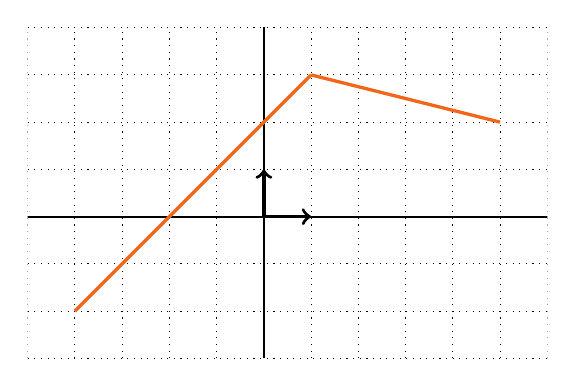
\begin{tikzpicture}[scale=0.6]
\clip (-5,-3) rectangle (6,4);
\draw [ thin, dotted] (-5,-3) grid (6,11);
\draw [thick] (-6,0)--(7,0);
\draw [thick] (0,-3)--(0,11);
\draw [->, very thick] (0,0)--(1,0);
\draw [->,very thick] (0,0)--(0,1);

\draw [ocre, very thick,domain=-4:1,samples=100] plot (\x,{\x+2});
\draw [ocre, very thick,domain=1:5,samples=100] plot (\x,{-0.25*\x+3.25});

\end{tikzpicture}\end{minipage}


\end{exercise}

\begin{solution}
 \(\displaystyle\int_{-2}^0f(x)\dx\) est l'aire d'un triangle et vaut \(\dfrac{2 \times 2}{2}=2\).

 \(\displaystyle\int_{0}^5f(x)\dx\) est l'aire de deux trapèzes. \\Le premier a une aire de \(\dfrac{(2+3)\times 1}{2}\) et le deuxième une aire de \(\dfrac{(3+2)\times 4}{2}\). L'aire total vaut donc \(12,5\).


 \(\displaystyle\int_{-1}^3f(x)\dx\) est l'aire de deux trapèzes. \\Le premier a une aire de \(\dfrac{(1+3) \times 2}{2}\) et le deuxième a une aire de \(\dfrac{(3+2.5)\times 2}{2}\). L'aire totale vaut donc 9,5.

 Pour calculer l'aire \(\displaystyle\int_{-2}^5f(x)\dx\), il suffit d'ajouter les aires \(\displaystyle\int_{-2}^0f(x)\dx\) et \(\displaystyle\int_{0}^5f(x)\dx\). L'aire recherchée vaut donc \(14,5\).\end{solution}



\begin{exercise}

\begin{minipage}{0.55\linewidth}
On considère la fonction $f$ dont la courbe représentative est donnée ci-contre dans un repère orthonormé.


Donner un encadrement de $\displaystyle\int_{-4}^5f(x)\dx$.

\end{minipage}\hfill\begin{minipage}{0.4\linewidth}
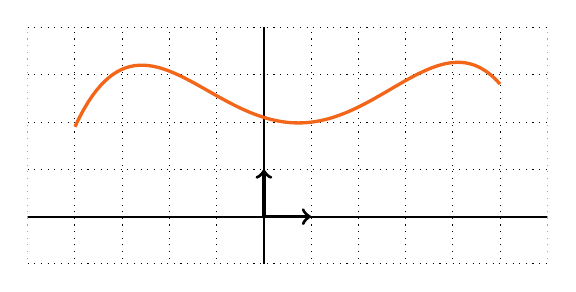
\begin{tikzpicture}[scale=0.6]
\clip (-5,-1) rectangle (6,4);
\draw [ thin, dotted] (-5,-3) grid (6,11);
\draw [thick] (-6,0)--(7,0);
\draw [thick] (0,-3)--(0,11);
\draw [->, very thick] (0,0)--(1,0);
\draw [->,very thick] (0,0)--(0,1);

\draw [ocre, very thick,domain=-4:5,samples=100] plot (\x,{-0.01*\x*\x*\x*\x+0.03*\x*\x*\x+0.19*\x*\x-0.31*\x+2.1});

\end{tikzpicture}\end{minipage}
\end{exercise}

\begin{solution}
Il est possible d'encadrer l'intégrale en comptant le nombre de carreaux sous la courbe pour avoir un minorant. On ajoute les carreaux que la courbe traverse pour obtenir un majorant. On a donc \(19 \leqslant \displaystyle\int_{-4}^5f(x)\dx \leqslant 30\). Cet encadrement peut largement être amélioré (en ne considérant que des demi-carreaux par exemple).
\end{solution}



\begin{exercise}Pour tout réel $x$, on pose $f(x)=2x+8$. Calculer $\displaystyle\int_{-3}^5 f(x)\dx$.\end{exercise}

\begin{solution}
Pour tout réel \(x\), on pose \(f(x)=2x+8\). \(\displaystyle\int_{-3}^5 f(x)\dx\) désigne l'aire ci-dessous.

\begin{center}
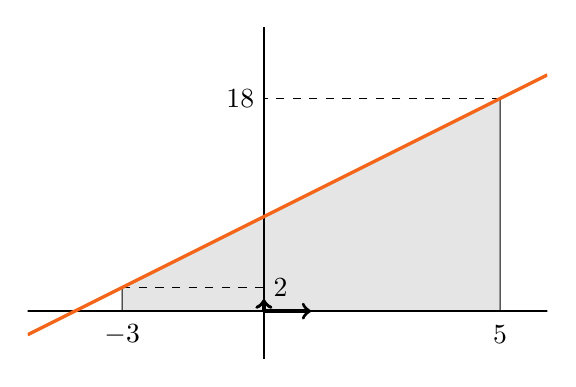
\begin{tikzpicture}[scale=0.6]
\clip (-5,-1) rectangle (6,6);
\filldraw[draw=black,fill=gray!20] plot [domain=-3:5] (\x,{\x/2+2}) -- (5,0)--(-3,0) --cycle;
\draw [thick] (-6,0)--(7,0);
\draw [thick] (0,-3)--(0,11);
\draw [->, very thick] (0,0)--(1,0);
\draw [->,very thick] (0,0)--(0,0.25);
\draw [dashed] (-3,1/2)--(0,1/2);
\draw (0,1/2) node[right] {$2$};

\draw [dashed] (5,9/2)--(0,9/2);
\draw (0,9/2) node[left] {$18$};

\draw [->,very thick] (0,0)--(0,0.25);
\draw (-3,-0.5) node {$-3$};
\draw (5,-0.5) node {$5$};

\draw [ocre, very thick,domain=-5:6,samples=100] plot (\x,{\x/2+2});

\end{tikzpicture}
\end{center}


Il s'agit de l'aire d'un trapèze dont les bases ont pour longueur 2 et 18 et la hauteur a pour longueur 8. Cette aire vaut donc \(\dfrac{(2+18)\times 8}{2}\). Ainsi,  \(\displaystyle\int_{-3}^5 f(x)\dx = \dfrac{2+18}{2} \times 8 = 80\).\end{solution}


\begin{exercise}On rappelle que pour tout réel $x$, $|x|= \max(x , -x)$. Déterminer $\displaystyle\int_{-3}^5 |x|\dx$.\end{exercise}

\begin{solution}

L'intégrale \(\displaystyle\int_{-3}^5 |x|\dx\) est représentée par l'aire ci-dessous.

\begin{center}
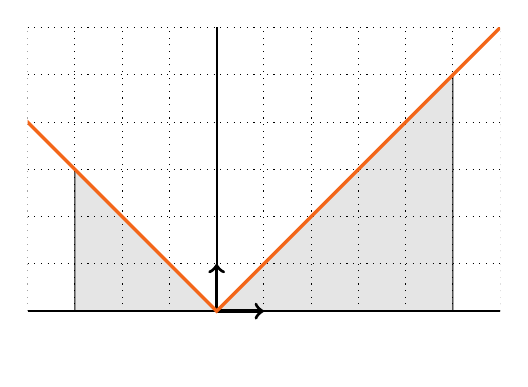
\begin{tikzpicture}[scale=0.6]
\clip (-4,-1) rectangle (6,6);
\filldraw[draw=black,fill=gray!20] (-3,3) -- (0,0)--(5,5) --(5,0) --(-3,0) --cycle;
\draw [ thin, dotted] (-4,0) grid (7.5,11);
\draw [thick] (-4,0)--(7.5,0);
\draw [thick] (0,0)--(0,11);
\draw [->, very thick] (0,0)--(1,0);
\draw [->,very thick] (0,0)--(0,1);

\draw [ocre, very thick,domain=-5:6,samples=100] plot (\x,{abs(\x)});


\end{tikzpicture}
\end{center}


Il s'agit de l'aire de deux triangles. Le premier a une aire de \(\dfrac{3\times 3}{2}\) et le deuxième une aire de \(\dfrac{5\times 3}{2}\). \\ Ainsi, \(\displaystyle\int_{-3}^5 |x|\dx = 17\).\end{solution}



\begin{exercise}Soit $x$ un réel supérieur ou égal à 4. Exprimer $\displaystyle\int_{4}^{x} (2t+3)dt$ en fonction de $x$.\end{exercise}

\begin{solution}

L'intégrale \(\displaystyle\int_{4}^{x} (2t+3)dt\) représente l'aire de la surface grisée ci-dessous.

\begin{center}
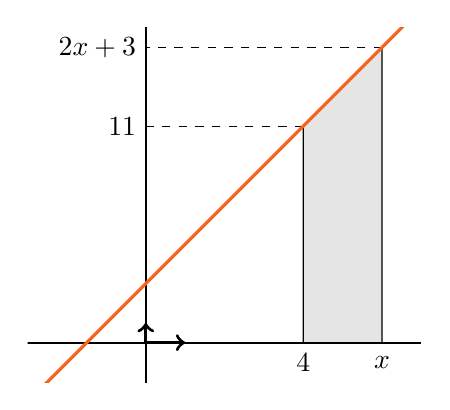
\begin{tikzpicture}[scale=0.5]
\clip (-3,-1) rectangle (7,8);
\filldraw[draw=black,fill=gray!20] plot [domain=4:6] (\x,{\x+1.5}) -- (6,0)--(4,0) --cycle;
\draw [thick] (-6,0)--(7,0);
\draw [thick] (0,-3)--(0,11);
\draw [->, very thick] (0,0)--(1,0);
\draw [->,very thick] (0,0)--(0,0.5);

\draw [dashed] (4,5.5)--(0,5.5);
\draw (0,5.5) node[left] {$11$};

\draw [dashed] (6,7.5)--(0,7.5);
\draw (0,7.5) node[left] {$2x+3$};

\draw (4,-0.5) node {$4$};
\draw (6,-0.5) node {$x$};

\draw [ocre, very thick,domain=-5:7,samples=100] plot (\x,{\x+1.5});

\end{tikzpicture}
\end{center}


Il s'agit de l'aire d'un trapèze dont les bases ont pour longueur 11 et \(2x+3\) et la hauteur a pour longueur \(x-4\). Cette aire vaut donc \(\dfrac{(2x+3+11)\times (x-4)}{2}\) soit \(x^2+3x-28\). Ainsi,  \(\displaystyle\int_{4}^{x} (2t+3)dt=x^2+3x-28\).

\end{solution}



\begin{exercise}Soit $f$ une fonction affine que l'on suppose positive sur $[-3;5]$, telle que $\displaystyle\int_{-3}^5 f(x)\dx=24$ et $\displaystyle\int_{1}^5 f(x)\dx=14$. Donner une expression de $f(x)$ pour tout réel $x$.\end{exercise}

\begin{solution}
Soit \(a\) et \(b\) deux réels tels que, pour tous réels  \(x\), \(f(x)=ax+b\). Représentons la situation.


\begin{center}
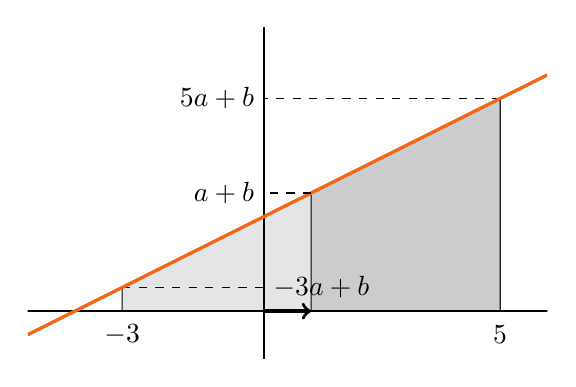
\begin{tikzpicture}[scale=0.6]
\clip (-5,-1) rectangle (6,6);
\filldraw[fill=gray!20] plot [domain=-3:5] (\x,{\x/2+2}) -- (5,0)--(-3,0) --cycle;
\filldraw[fill=gray!40] plot [domain=1:5] (\x,{\x/2+2}) -- (5,0)--(1,0) --cycle;
\draw [thick] (-6,0)--(7,0);
\draw [thick] (0,-3)--(0,11);
\draw [->, very thick] (0,0)--(1,0);

\draw [dashed] (-3,1/2)--(0,1/2);
\draw (0,1/2) node[right] {$-3a+b$};

\draw [dashed] (5,9/2)--(0,9/2);
\draw (0,9/2) node[left] {$5a+b$};
\draw (-3,-0.5) node {$-3$};
\draw (5,-0.5) node {$5$};
\draw [ocre, very thick,domain=-5:6,samples=100] plot (\x,{\x/2+2});
\draw [dashed] (1,5/2)--(0,5/2);
\draw (0,5/2) node[left] {$a+b$};
\end{tikzpicture}
\end{center}

L'aire \(\displaystyle\int_{-3}^5 f(x)\dx\) correspond à l'aire jointe des deux trapèzes. \\ Celle-ci vaut \(\dfrac{-3a+b+5a+b}{2} \times (5-(-3))=8(a+b)\).

L'aire \(\displaystyle\int_{1}^5 f(x)\dx\) correspond à l'aire du trapèze foncé. Celle-ci vaut \(\dfrac{a+b+5a+b}{2} \times (5-1)=2(6a+2b)\).

Ainsi, on a \(\displaystyle\int_{-3}^5 f(x)\dx=24\) et \(\displaystyle\int_{1}^5 f(x)\dx=14\) si et seulement si  \(\left\{\begin{array}{l} 8(a+b) = 24 \\ 2(6a+2b)=14\end{array}\right.\).

Ce système est équivalent à \(\left\{\begin{array}{l} a+b = 3 \\ 6a+2b=7\end{array}\right.\).

En soustrayant deux fois la première ligne à la deuxième ligne, on obtient \(\left\{\begin{array}{l} a+b = 3 \\ 4a=1\end{array}\right.\).

Finalement, \(\left\{\begin{array}{l} b = \frac{11}{4} \\ a=\frac{1}{4}\end{array}\right.\). Ainsi, pour tout réel \(x\), \(f(x)=\dfrac{x}{4}+\dfrac{11}{4}\).

\end{solution}



\begin{exercise}Soit $f$ la fonction définie pour tout réel $x \in [0;1]$ par $f(x)=\sqrt{1-x^2}$. Après avoir déterminé la nature de la courbe représentative de $f$, déterminer la valeur de $\displaystyle\int_{-1}^1 f(x)\dx$.\end{exercise}

\begin{solution}

La courbe représentative de la fonction $x\mapsto \sqrt{1-x^2}$ sur $[-1;1]$ est le demi-cercle supérieur de centre $O$ et de rayon 1. L'aire du demi-disque vaut $\dfrac{\pi}{2}$. Ainsi, $\displaystyle\int_{-1}^1  \sqrt{1-x^2}\dx=\dfrac{\pi}{2}$.
\begin{center}
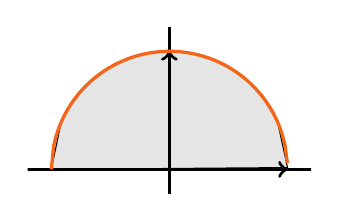
\begin{tikzpicture}[scale=1.5]
\clip (-1.2,-0.2) rectangle (1.2,1.2);
\filldraw[draw=black,fill=gray!20] plot [domain=-1:1] (\x,{sqrt(1-\x*\x)})  --cycle;
\draw [thick] (-6,0)--(7,0);
\draw [thick] (0,-3)--(0,11);
\draw [->, very thick] (0,0)--(1,0);
\draw [->,very thick] (0,0)--(0,1);


\draw [ocre, very thick,domain=-1:1,samples=100] plot (\x,{sqrt(1-\x*\x)});

\end{tikzpicture}
\end{center}



\end{solution}




\section*{Intégrale et primitives}



 \begin{exercise}Calculer les intégrales suivantes.  \renewcommand{\arraystretch}{2.5}
 \vspace{-0.5cm}
 \begin{center}
 \begin{tabularx}{\linewidth}{XXX}
 \textbf{a.} $\displaystyle\int_{-5}^{7} \sqrt{2} \dx$ &
 \textbf{b.} $\displaystyle\int_{3}^{14} \dfrac{1}{x} \dx$&
 \textbf{c.} $\displaystyle\int_{-2}^4 (x^2+3x+4) \dx$ \\
 \textbf{d.} $\displaystyle\int_{0}^{10} \e^{-5x} \dx$ &
 \textbf{e.}  $\displaystyle\int_{-1}^{1} (x^4-x^2+x-1) \dx$&
 \textbf{f.}    $\displaystyle\int_{-2}^{2} (8x^5+5x^3+2x) \dx$\\
 \textbf{g.} $\displaystyle\int_{0}^1 \e^{2x} \dx$&
  
 \textbf{h.} $\displaystyle\int_{1}^{9} \dfrac{3}{2\sqrt{x}} \dx$ &
 \textbf{i.} $\displaystyle\int_{0}^{2} \left((x+1)(x+2)\right) \dx$ \\
 \textbf{j.} $\displaystyle\int_{0}^{1} \dfrac{1}{1+x} \dx$ & \textbf{k.} $\displaystyle\int_3^7 \dfrac{1}{x^2}\dx$ & \textbf{l.} $\displaystyle\int_1^2 \dfrac{x+1}{x^3}\dx$
 \end{tabularx}\end{center}\end{exercise}

\begin{solution}

\textbf{a.} \(\displaystyle\int_{-5}^{7} \sqrt{2} \dx = [\sqrt{2}x]_{-5}^7=\sqrt{2}(7-(-5))=12\sqrt{2}\). Il est aussi possible de procéder à un calcul d'aire.

\textbf{b.} \(\displaystyle\int_{3}^{14} \dfrac{1}{x} \dx = [\ln(x)]_3^{14}=\ln(14)-\ln(3)=\ln\left(\dfrac{14}{3}\right)\).

\textbf{c.}  \(\displaystyle\int_{-2}^4 (x^2+3x+4) \dx = \left[\dfrac{x^3}{3}+\dfrac{3}{2}x^2+4x\right]_{-2}^4= \dfrac{4^3}{3}+\dfrac{3}{2}\times 4^2 + 4 \times 4 -\left( \dfrac{(-2)^3}{3}+\dfrac{3}{2}\times (-2)^2+4\times (-2)\right)=66\).

\textbf{d.} \(\displaystyle\int_{0}^{10} \e^{-5x} \dx = \left[ \dfrac{\e^{-5x}}{-5}\right]_0^{10}= -\dfrac{\e^{-50}}{5}+\dfrac{1}{5}\). Attention à d'éventuelles erreurs de signe ici !

\textbf{e.} \(\displaystyle\int_{-1}^{1} (x^4-x^2+x-1) \dx = \left[\dfrac{x^5}{5}-\dfrac{x^3}{3}+\dfrac{x^2}{2}-x\right]_{-1}^{1}=-\dfrac{34}{15}\).

\textbf{f.} \(\displaystyle\int_{-2}^{2} (8x^5+5x^3+2x) \dx = \left[\dfrac{4}{3}x^6+\dfrac{5}{4}x^4+x^2\right]_{-2}^2=0\). On aurait également pu tout simplement remarquer que la fonction intégrée était impaire et l'intervalle d'intégration symétrique par rapport à 0.

\textbf{g.} \(\displaystyle\int_{0}^1 \e^{2x} \dx=\left[\dfrac{\e^{2x}}{2}\right]_0^1=\dfrac{\e^2-1}{2}\).

\textbf{h.} \(\displaystyle\int_{1}^{9} \dfrac{3}{2\sqrt{x}} \dx = \left[3\sqrt{x}\right]_1^9=6\).

\textbf{i.}  \(\displaystyle\int_{0}^{2} \left((x+1)(x+2)\right) \dx = \displaystyle\int_{0}^{2} (x^2+3x+2)\dx = \left[\dfrac{x^3}{3}+\dfrac{3x^2}{2}+2x\right]_0^2 = \dfrac{38}{3}\).

\textbf{j.} \(\displaystyle\int_{0}^{1} \dfrac{1}{1+x} \dx = \left[ \ln(1+x) \right]_0^1=\ln(2)\).

\textbf{k.} \(\displaystyle\int_3^7 \dfrac{1}{x^2}\dx = \left[-\dfrac{1}{x}\right]_3^7 = \dfrac{4}{21}\).

\textbf{l.} \(\displaystyle\int_1^2 \dfrac{x+1}{x^3}\dx = \displaystyle\int_1^2 \left(\dfrac{1}{x^2}+\dfrac{1}{x^3}\right)\dx = \left[-\dfrac{1}{x}-\dfrac{1}{2x^2}\right]_1^2 = \dfrac{7}{8} \).
\end{solution}
 
 

 \begin{exercise}Calculer les intégrales suivantes.
 \renewcommand{\arraystretch}{2.5}
  \vspace{-0.5cm}
 \begin{center}
 \begin{tabularx}{\linewidth}{XXX}
 \textbf{a.} $\displaystyle\int_{-2}^4 2x\e^{x^2} \dx$ & \textbf{b.} $\displaystyle\int_{2}^{e} \dfrac{1}{x\ln(x)}\dx$ &
\textbf{c.} $\displaystyle\int_{1}^{3} \dfrac{\e^{1/x}}{x^2} \dx$ \\
\textbf{d.} $\displaystyle\int_{0}^{4} \dfrac{2x}{1+x^2} \dx$&
\textbf{e.} $\displaystyle\int_{-1}^{4} \dfrac{x}{\sqrt{9+x^2}} \dx$ & \textbf{f.} $\displaystyle\int_{-3}^2 \dfrac{\e^x}{(1+\e^x)^2}\dx$
 \end{tabularx}\end{center}\end{exercise}
 
 \begin{solution}

\textbf{a.} Pour tout réel \(x \in [-2;4]\), on pose \(u(x)=x^2\). On a alors \(u'(x)=2x\) et \(2x\e^{x^2} = u'(x) \times \e^{u(x)}\). Une primitive de \(x\mapsto 2x\e^{x^2}\) sur \([-2;4]\) est donc la fonction \(x \mapsto \e^{x^2}\). Ainsi, \[\displaystyle\int_{-2}^4 2x\e^{x^2} \dx=\left[\e^{x^2}\right]_{-2}^4=\e^{16}-\e^4.\]

\textbf{b.} Pour tout réel \(x \in [2;e]\), on pose \(u(x)=\ln(x)\) (qui est alors strictement positif). On a alors \(u'(x)=\dfrac{1}{x}\) et \(\dfrac{1}{x\ln(x)} = \dfrac{\frac{1}{x}}{\ln(x)} = \dfrac{u'(x)}{u(x)}\). Une primitive de \(x\mapsto \dfrac{1}{x\ln(x)}\) sur \([2;e]\) est donc la fonction \(x \mapsto \ln(\ln(x))\). Ainsi, \[\displaystyle\int_{2}^e \dfrac{1}{x\ln(x)} \dx=\left[\ln \ln (x)\right]_{2}^e=-\ln(\ln(2)).\]

\textbf{c.} Pour tout réel \(x \in [1;3]\), on pose \(u(x)=\dfrac{1}{x}\). On a alors \(u'(x)=-\dfrac{1}{x^2}\) et \(\dfrac{\e^{1/x}}{x^2} = - \left(-\dfrac{1}{x^2}\right)\e^{1/x} = -u'(x) \times \e^{u(x)}\). Une primitive de \(x\mapsto \dfrac{\e^{1/x}}{x^2}\) sur \([1;3]\) est donc la fonction \(x \mapsto -\e^{1/x}\). Ainsi, \[\displaystyle\int_{1}^{3} \dfrac{\e^{1/x}}{x^2} \dx=\left[-\e^{1/x}\right]_{1}^3=e-\e^{1/3}.\]

\textbf{d.} Pour tout réel \(x \in [0;4]\), on pose \(u(x)=1+x^2\). On a alors \(u'(x)=2x\) et \(\dfrac{2x}{1+x^2} = \dfrac{u'(x)}{u(x)}\). Une primitive de \(x\mapsto \dfrac{2x}{1+x^2}\) sur \([0;4]\) est donc la fonction \(x \mapsto \ln (1+x^2)\). Ainsi, \[\displaystyle\int_{0}^{4} \dfrac{2x}{1+x^2} \dx=\left[\ln(1+x^2)\right]_0^4=\ln(17).\]

\textbf{e.} Pour tout réel \(x \in [-1;4]\), on pose \(u(x)=9+x^2\). On a alors \(u'(x)=2x\) et \(\dfrac{x}{\sqrt{9+x^2}}=\dfrac{2x}{2\sqrt{9+x^2}} = \dfrac{u'(x)}{2\sqrt{u(x)}}\). Une primitive de \(x\mapsto \dfrac{x}{\sqrt{9+x^2}}\) sur \([-1;4]\) est donc la fonction \(x \mapsto \sqrt{9+x^2}\). Ainsi, \[\displaystyle\int_{-1}^{4} \dfrac{x}{\sqrt{9+x^2}} \dx=\left[\sqrt{9+x^2}\right]_{-1}^4=5-\sqrt{10}.\]

\textbf{f.} Pour tout réel \(x \in [-3;2]\), on pose \(u(x)=1+\e^x\). On a alors \(u'(x)=\e^x\) et \(\dfrac{\e^x}{(1+\e^x)^2} = -\dfrac{u'(x)}{u(x)^2}\). Une primitive de \(x\mapsto \dfrac{\e^x}{(1+\e^x)^2}\) sur \([-3;2]\) est donc la fonction \(x \mapsto -\dfrac{1}{1+\e^x}\). Ainsi, \[\displaystyle\int_{-3}^{2} \dfrac{\e^x}{(1+\e^x)^2} \dx=\left[-\dfrac{1}{1+\e^x}\right]_{-3}^2=\dfrac{1}{1+\e^{-3}}-\dfrac{1}{1+\e^2}.\]
\end{solution}


 
  
 \begin{exercise}
Pour tout réel $x> -1$, on pose $f(x)=\dfrac{x}{(x+1)^2}$.

\begin{enumerate}
\item Montrer que pour tout réel $x>-1$, $f(x)=\dfrac{1}{x+1}-\dfrac{1}{(x+1)^2}$.
\item En déduire une primitive de $f$ sur $]-1;+\infty[$.
\item Calculer alors $\displaystyle\int_{1}^3 f(x)\dx$.
\end{enumerate}\end{exercise}


\begin{solution}
Pour tout réel \(x>-1\), 
\[\dfrac{1}{x+1}-\dfrac{1}{(x+1)^2}=\dfrac{(x+1)-1}{(x+1)^2}=\dfrac{x}{(x+1)^2}=f(x).\]
Une primitive de \(f\) sur \(]-1;+\infty[\) est donc \(F:x\mapsto \ln(x+1)+\dfrac{1}{x+1}\).

Ainsi, \(\displaystyle\int_{1}^3 f(x)\dx = \left[ \ln(x+1)+\dfrac{1}{x+1} \right]_1^3=\ln(4)+\dfrac{1}{4}-\ln(2)-\dfrac{1}{2}=\ln(2)-\dfrac{1}{4}\).
\end{solution}


\begin{exercise}

    Un cycliste roule sur une route descendante rectiligne et très longue. 
    
    On note $v(t)$ sa vitesse à l'instant $t$ , où $t$ est exprimé en secondes et $v(t)$ en mètres par seconde.

On suppose de plus que la fonction $v$ ainsi définie est dérivable sur l'intervalle $[0;+\infty [$.


\paragraph{Partie A : Résolution d'une équation différentielle}

Un modèle simple permet de considérer que la fonction $v$ est solution de l'équation différentielle (E) suivante :
\[(E) \quad : \quad 10y'+y=30\]

\begin{enumerate}
    \item Résoudre l'équation homogène associée $(H)$ : $10y'+y=0$.
    \item Déterminer une solution constante de l'équation $(E)$.
    \item En déduire l'ensemble des solutions de l'équation $(E)$.
    \item On suppose que, lorsque le cycliste s'élance, sa vitesse initiale est nulle. On a donc $v(0) = 0$. \\ Déterminer une expression de $v(t)$ pour tout réel $t\geqslant 0$.
\end{enumerate}

\paragraph{Partie B : Étude de la fonction $v$}

On considère la fonction $v:t\mapsto 30-30\exp\left(-\dfrac{t}{10}\right)$.
\begin{enumerate}
    \item Montrer que la fonction $v$ est croissante et concave sur $[0;+\infty[$.
    \item Déterminer la limite de la fonction $v$ en $+\infty$.
    \item On considère, dans cette situation, que la vitesse du cycliste est stabilisée lorsque son accélération $v'(t)$ est inférieure à 0,1 m.s$^{-2}$. 
\begin{enumerate}
\item Compléter le programme suivant, écrit en Python, qui permet de renvoyer la plus petite valeur de $t$, à la seconde près, à partir de laquelle la vitesse du cycliste est stabilisée. On rappelle que la commande \textbf{from math import exp }permet d'utiliser la fonction exponentielle qui s'écrit \textbf{exp} en Python.

\begin{lstlisting}[language=python]
from math import exp

def v_prime(x) :
	return ...
	
def seuil() :
	t = 0
	while v_prime(t) ... :
		t = ...	
	return t
\end{lstlisting}

\item A l'aide d'une résolution d'inéquation, déterminer la valeur de $t$ recherchée.
\end{enumerate}
   
    \item La distance $d$ parcourue par ce cycliste entre les instants $t_1$, et $t_2$ est donnée par $d=\displaystyle\int_{t_1}^{t_2}v(t)\dt$.\\
    Calculer la distance parcourue par ce cycliste pendant les 35 premières secondes, arrondie au mètre près.
\end{enumerate}

\end{exercise}

\begin{solution}

\textbf{Partie A : Résolution d'une équation différentielle}
\begin{enumerate}
\item On a $10y'+y=0$ si et seulement si $y'+\dfrac{1}{10}y=0$. Les solutions de cette équation sont les fonctions $t\mapsto C\e^{-t/10}$, pour $C$ réel.
\item La solution constante de l'équation $(E)$ est $y=30$.
\item L'ensemble des solutions de $(E)$ est donc l'ensemble des fonctions de la forme $t\mapsto C\e^{-t/10}+30$, pour $C$ réel.
\item On cherche $C$ tel que $v(0)=0$. On a alors $C+30=0$ et donc $C=-30$. Ainsi, pour tout réel $t$, on a $v(t)=-30\e^{-t/10}+30=30(1-\e^{-t/10})$.
\end{enumerate}

\textbf{Partie B : Étude de la fonction $v$}


\begin{enumerate}
\item Pour tout réel $t\geqslant 0$, on a $v'(t)=3\exp\left(-\dfrac{t}{10}\right)$ et $v''(t)=-\dfrac{3}{10}\exp\left(-\dfrac{t}{10}\right)$. En particulier, pour tout réel $t\geqslant 0$, on a $v'(t)\geqslant 0$ et $v''(t)\leqslant 0$. La fonction $v$ est donc croissante et concave sur $]0;+\infty[$.
\item On a $\displaystyle\lim_{t \to +\infty}\left(-\dfrac{t}{10}\right)=-\infty$ et $\displaystyle\lim_{T \to -\infty}\exp(T)=0$. Ainsi, par composition $\displaystyle\lim_{t\to +\infty}\exp\left(-\dfrac{t}{10}\right)=0$ et donc $\displaystyle\lim_{t\to +\infty}v(t)=30$.
\item 
\begin{enumerate}
\item On complète le programme Python ci-dessous.
\begin{lstlisting}[language=python]
from math import exp

def v_prime(x) :
	return 3 * exp(-x/10)
	
def seuil() :
	t = 0
	while v_prime(t) > 0.1 :
		t = t + 1
	return t
\end{lstlisting}
\item on cherche la plus petite valeur entière de $t$ pour laquelle  $v'(t) \leqslant 0.1$. Or, $v'(t)\leqslant 0,1$ si et seulement si $3\exp\left(-\dfrac{t}{10}\right) \leqslant 0,1$ soit $\left(-\dfrac{t}{10}\right) \leqslant \dfrac{1}{30}$. Par croissance de la fonction logarithme népérien sur $]0;+\infty[$, cela équivaut à $-\dfrac{t}{10}\leqslant \ln\left(\dfrac{1}{30}\right)$ soit $t \geqslant 10\ln(30)$. Or, $10\ln(30) \simeq 34,01$. La valeur recherchée est donc 35 secondes.

\end{enumerate}
\item Une primitive de $v$ sur $[0;+\infty[$ est $V:t\mapsto 30t+300\exp\left(-\dfrac{t}{10}\right)$. Ainsi, $\displaystyle\int_0^{35}v(t)=[V(t)]_0^{35}\simeq 759$.
\end{enumerate}

\end{solution}

 
\begin{exercise}On considère la fonction $f$ définie pour tout réel $x$ par $f(x)=\left\{\renewcommand{\arraystretch}{1}\begin{array}{ll} x^2+x&,\text{ si }x<-1\\ 2x^3-x+1&,\text{ si }x\geqslant -1\end{array}\right.$.

 Justifier que $f$ est continue sur $[-4;1]$ puis calculer $\displaystyle\int_{-4}^1 f(t)dt$.\end{exercise}


\begin{solution}

Le seul problème éventuel se situe en \(-1\). On a \(\displaystyle\lim_{x \to -1^1}f(x)=(-1)^2+(-1)=0\) et \\ \(\displaystyle\lim_{x \to -1^+}f(x)=2 \times (-1)^3-(-1)+1=0\). Ainsi, \(f\) est continue sur \([-4;1]\). 

 D'après la relation de Chasles,\[\displaystyle\int_{-4}^1 f(t)dt = \displaystyle\int_{-4}^{-1} f(t)dt+\displaystyle\int_{-1}^1 f(t)dt = \displaystyle\int_{-4}^{-1} (t^2+t)dt
+\displaystyle\int_{-1}^1 (2t^3-t+1)dt .\]

Or, \( \displaystyle\int_{-4}^{-1} (t^2+t)dt = \left[ \dfrac{t^3}{3}+\dfrac{t^2}{2}\right]_{-4}^{-1}=\dfrac{27}{2}\) et \(\displaystyle\int_{-1}^1 (2t^3-t+1)d=\left[\dfrac{t^4}{2}-\dfrac{t^2}{2}+t\right]_{-1}^1=2\).

Ainsi, \(\displaystyle\int_{-4}^1 f(t)dt=\dfrac{31}{2}\).\end{solution} 



\begin{exercise}
 \begin{minipage}{0.7\linewidth}
 On a tracé ci-contre, dans un repère orthonormé, les courbes des fonctions $f :x\mapsto x^2$ et $g:x \mapsto x^3$ sur l'intervalle $[0;1]$.
\begin{enumerate}
\item Justifier que, pour tout réel $x\in [0;1]$, $f(x)\geqslant g(x)$.
\item Calculer l'aire de la surface grisée.
\end{enumerate}

\end{minipage}\hfill \begin{minipage}{0.25\linewidth}
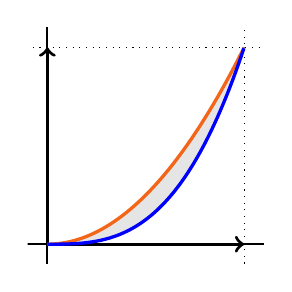
\begin{tikzpicture}[scale=2.5]
\clip (-0.1,-0.1) rectangle (1.1,1.1);
\filldraw[draw=black,fill=gray!20] plot [domain=0:1] (\x,{\x*\x}) -- plot [domain=1:0] (\x,{\x*\x*\x}) --cycle;
\draw [ thin, dotted] (-5,-3) grid (6,11);
\draw [thick] (-6,0)--(7,0);
\draw [thick] (0,-3)--(0,11);
\draw [->, very thick] (0,0)--(1,0);
\draw [->,very thick] (0,0)--(0,1);
\draw [ocre, very thick,domain=0:1,samples=100] plot (\x,{\x*\x});
\draw [blue, very thick,domain=0:1,samples=100] plot (\x,{\x*\x*\x});


\end{tikzpicture}\end{minipage}
\end{exercise}

\begin{solution}
On a \[\displaystyle \int_{0}^1 \dfrac{\e^x}{1+\e^x}\dx +  \int _0^1 \dfrac{1}{1+\e^x}\dx = \int _0^1 \dfrac{1+\e^x}{1+\e^x}\dx = \int _0^1 1\dx = 1 .\]

Par ailleurs, si on pose pour tout \(x\in [0,1]\), \(u(x)=1+\e^x\), on a \(\dfrac{\e^x}{1+\e^x}=\dfrac{u'(x)}{1+u(x)}\). \(u\) étant strictement positive, une primitive de \(x \mapsto \dfrac{\e^x}{1+\e^x}\) sur \([0;1]\) est la fonction \(x \mapsto \ln(1+\e^x)\). Ainsi, 
\[\displaystyle \int_{0}^1 \dfrac{\e^x}{1+\e^x}\dx = \left[ \ln(1+\e^x)\right]_0^1 = \ln(1+e)-\ln(2)=\ln\left(\dfrac{1+e}{2}\right) .\]

Finalement, 
\[  \int _0^1 \dfrac{1}{1+\e^x}\dx = 1 - \ln\left(\dfrac{1+e}{2}\right) = \ln(e)-\ln\left(\dfrac{1+e}{2}\right) = \ln\left(\dfrac{2e}{1+e}\right) .\]

\end{solution}



\begin{exercise}Déterminer la valeur de $\displaystyle\int _0^1 \dfrac{1}{1+\e^x}\dx$ en utilisant celle de $\displaystyle \int_{0}^1 \dfrac{\e^x}{1+\e^x}\dx +  \int _0^1 \dfrac{1}{1+\e^x}\dx$.\end{exercise}

\begin{solution}
Soit \(x\in[0;1]\). On a alors \(0\leqslant x \leqslant 1\) puis, en multipliant cette inégalité par \(x^2\), \(0\leqslant x^3 \leqslant x^2\), et donc \(g(x)\leqslant f(x)\).

L'aire de la surface grisée vaut \[\int_0^1 (f-g)(x)\dx = \int_0^1 (x^2-x^3)\dx = \left[\dfrac{x^3}{3}-\dfrac{x^4}{4}\right]_0^1=\dfrac{1}{3}-\dfrac{1}{4}=\dfrac{1}{12}.\]
\newpage \end{solution}



\begin{exercise}
Pour tout entier naturel  $n$, on pose $u_n=\displaystyle \int _{0}^n\e^{-x^2}\dx$.
\begin{enumerate}
\item Montrer que la suite $(u_n)$ est croissante.
\item Montrer que pour tout réel $x\geqslant 0$, on a $-x^2 \leqslant -2x+1$ et que $\e^{-x^2}\leqslant \e^{-2x+1}$.
\item En déduire que pour tout entier naturel $n$, $u_n \leqslant \dfrac{e}{2}$.
\item En déduire que la suite $(u_n)$ converge. On ne cherchera pas à calculer sa limite.
\end{enumerate}\end{exercise}

\begin{solution}\hspace{0pt}
\begin{enumerate}
\item  Pour tout entier naturel \(n\)
\[ u_{n+1}-u_n = \displaystyle \int _{0}^{n+1}\e^{-x^2\dx}-\displaystyle \int _{0}^n\e^{-x^2\dx}=\displaystyle \int _{n}^{n+1}\e^{-x^2}\dx.\]
Puisque pour tout réel \(x\) entre \(n\) et \(n+1\), \(\e^{-x^2}>0\), il en vient que \(\int _{n}^{n+1}\e^{-x^2}\dx \geqslant 0\) et donc \(u_{n+1} \geqslant u_n\). La suite \((u_n)\) est croissante.
\item  Soit \(x\geqslant 0\). Alors \((x-1)^2\geqslant 0\), c'est-à-dire, \(x^2-2x+1 \geqslant 0\) et donc \(-x^2 \leqslant -2x+1\). La fonction exponentielle étant croissante, on a alors \(\e^{-x^2}\leqslant \e^{-2x+1}\).
\item  Ainsi, pour tout entier naturel \(n\),
\[u_n=\int _{0}^n\e^{-x^2}\dx \leqslant \int _{0}^n\e^{-2x+1}\dx = \left[\dfrac{\e^{-2x+1}}{-2}\right]_0^n=-\dfrac{\e^{2n+1}}{2}+\dfrac{e}{2}\leqslant \dfrac{e}{2}.\]

\item  La suite \((u_n)\) est croissante et majorée : cette suite est donc convergente.
\end{enumerate}\end{solution}



\begin{exercise}Déterminer la valeur moyenne de la fonction $f:x\mapsto 3x+2$ sur $[-2;3]$.\end{exercise}

\begin{solution}
La valeur moyenne de la fonction \(f:x\mapsto 3x+2\) sur \([-2;3]\) vaut
\[ \dfrac{1}{3-(-2)}\int_{-2}^3(3x+2)\dx = \dfrac{1}{5}\left[\dfrac{3}{2}x^2+2x\right]_{-2}^3=\dfrac{7}{2}.\]\end{solution}



\begin{exercise}Déterminer la valeur moyenne de la fonction $f:x\mapsto -x^2+4x$ sur $[0;4]$.\end{exercise}

\begin{solution}
La valeur moyenne de la fonction \(f:x\mapsto -x^2+4x\) sur \([0;4]\) vaut
\[ \dfrac{1}{4-(0)}\int_{0}^4(-x^2+4x)\dx = \dfrac{1}{4}\left[-\dfrac{x^3}{3}+2x^2\right]_{0}^4=-\dfrac{64}{3}+32 = \dfrac{1}{4}\times \dfrac{32}{3} = \dfrac{8}{3}.\]
\end{solution}


\begin{exercise}Un bénéfice, en milliers d'euros, que réalise une entreprise lorsqu'elle fabrique $x$ milliers de pièces est égal à :
\[f(x)=\dfrac{5 \ln(x)}{x} +3.\]

\begin{enumerate}
\item Montrer que $F: x \mapsto \dfrac{5 \ln(x)^2}{2}+3x$ est une primitive de $f$ sur $[2;4]$.
\item Calculer la valeur moyenne du bénéfice lorsque la production varie de 2000 à 4000 pièces.
\end{enumerate}

\end{exercise}

\begin{solution}

 On rappelle que si \(u\) est dérivable sur un intervalle \(I\), alors \(u^2\) l'est également et \((u^2)'=2u'u\). Pour tout réel \(x\in[2;4]\), 
	\[F'(x)=\dfrac{5}{2} \times 2 \times \dfrac{1}{x} \times \ln (x) + 3 = f(x).\]
\(F\) est donc une primitive de \(f\) sur \([2;4]\).

La valeur moyenne du bénéfice lorsque la production varie de 2000 à 4000 pièces vaut
\[\dfrac{1}{4-2}\int_{2}^{4} f(x)\dx = \dfrac{1}{2}\left[F(x)\right]_{2}^4 = \dfrac{1}{2} \times \left(\dfrac{5 \ln(4)^2}{2}+3 \times 4 - \dfrac{5 \ln(2)^2}{2}-3\times 2\right).\]
	En utilisant le fait que \(\ln(4) = 2 \ln(2)\), on obtient
\[ \dfrac{1}{4-2}\int_{2}^{4} f(x)\dx = 3 + \dfrac{15\ln(2)^2}{4}.\]
\newpage
\end{solution}




\begin{exercise}Soit $f$ une fonction affine. Montrer que la valeur moyenne de $f$ sur l'intervalle $[a,b]$ vaut $\dfrac{f(a)+f(b)}{2}$.\end{exercise}

\begin{solution}

Soit \(m\) et \(p\) les réels tels que, pour tout réel \(x\), \(f(x)=mx+p\). La valeur moyenne de \(f\) sur \([a;b]\) vaut
\[\dfrac{1}{b-a} \int_a^b (mx+p)\dx = \dfrac{1}{b-a} \left[\dfrac{mx^2}{2}+px\right]_a^b = \dfrac{1}{b-a} \times \left(\dfrac{mb^2-ma^2}{2}+p(b-a)\right)\]
puis
\[\dfrac{1}{b-a} \int_a^b (mx+p)\dx = \dfrac{1}{b-a} \times (b-a) \times \left(\dfrac{m(b+a)+2p}{2}\right)\]
et donc
\[\dfrac{1}{b-a} \int_a^b (mx+p)\dx =  \dfrac{mb+ma+2p}{2} = \dfrac{ma+p+mb+p}{2}=\dfrac{f(a)+f(b)}{2}.\]
\end{solution}




\section*{Intégration par parties}


\begin{exercise}
A l'aide d'une intégration par parties, calculer $\displaystyle\int_{1}^4 x\ln(x)\dx$. On pourra poser $v=\ln$ et déterminer une fonction $u$ tel que pour tout réel $x$, $u'(x)=x$.\end{exercise}

\begin{solution}
Pour tout réel \(x\in[1;4]\), on pose...
\begin{itemize}
\item  \(v(x)=\ln(x)\). On a alors \(v'(x)=\dfrac{1}{x}\) ;
\item  \(u(x)=\dfrac{x^2}{2}\) de sorte que \(u'(x)=\dfrac{x^2}{2}\).
\end{itemize}

On souhaite alors calculer \(\displaystyle\int_{1}^4 (u'v)(x)\dx\). D'après la formule d'intégration par parties,
\[ \displaystyle\int_{1}^4 (u'v)(x)\dx = [uv]_1^4 - \displaystyle\int_{1}^4 (uv')(x)\dx=\left[\dfrac{x^2}{2}\ln(x)\right]_1^4-\displaystyle\int_{1}^4 \dfrac{x^2}{2} \times \dfrac{1}{x}\dx=8\ln(4)- \left[ \dfrac{x^2}{4}\right]_1^4 = 8\ln(4)-\dfrac{15}{4}.\]\end{solution}



\begin{exercise}[subtitle={(Un extrait d'exercice que j'ai eu au bac...)}]
On note $I=\displaystyle\int_1^e \ln(x) \dx$ et $J=\displaystyle\int_1^e (\ln(x))^2\dx$.
\begin{enumerate}
\item Vérifier que la fonction $F$ définie sur l'intervalle $]0;+\infty[$ par $F(x)=x\ln(x)-x$ est une primitive de la fonction logarithme népérien sur cet intervalle.
\item En déduire la valeur de $I$.
\item À l'aide d'une intégration par parties, déterminer la valeur de $J$.
\end{enumerate}
\end{exercise}

\begin{solution}$F$ est dérivable sur $]0;+\infty[$ et, pour tout réel $x>0$, $F'(x)=1\times \ln(x)+x \times \dfrac{1}{x} - 1 = \ln(x)$. $F$ est donc bien une primitive de $\ln$ sur $]0;+\infty[$.

Ainsi, $I=\displaystyle\int_1^e \ln(x)\dx = [x\ln(x)-x]_1^e = e\ln(e) - e -(1\ln(1)-1) = 1$.

Pour tout réel \(x\in[1;e]\), on pose...
\begin{itemize}
\item  \(v(x)=\ln(x)\). On a alors \(v'(x)=\dfrac{1}{x}\) ;
\item  \(u(x)=x\ln(x)-x\) de sorte que \(u'(x)=\ln(x)\).
\end{itemize}

On souhaite alors calculer \(J=\displaystyle\int_{1}^e (u'v)(x)\dx\). D'après la formule d'intégration par parties,
\[ J = [(x\ln(x)-x)\ln(x)]_1^e - \displaystyle\int_1^e \dfrac{x\ln(x)-x}{x}\dx = 0 - \displaystyle\int_1^e(\ln(x)-1).\]
Ainsi,
\[J=-\left(\displaystyle\int_1^e\ln(x)\dx-\displaystyle\int_1^e 1\dx\right) = -I+(e-1)=e-2.\]
\end{solution}



\begin{exercise}
Soit $t$ un réel strictement supérieur à 1. A l'aide d'une intégration par parties, calculer $\displaystyle\int_{1}^t \ln(x)\dx$. On pourra poser $v=\ln$ et déterminer une fonction $u$ tel que pour tout réel $x$, $u'(x)=1$.\end{exercise}

\begin{solution}
	Pour tout réel \(x \in [0;1]\), on pose \(v(x)=\ln(x)\) et \(u(x)=x\). Ainsi, par intégration par parties,
	\[\displaystyle\int_{1}^t \ln(x)\dx = \displaystyle\int_{1}^t u'(x)v(x)\dx = \left[uv\right]_1^t-\displaystyle\int_{1}^t u(x)v'(x)\dx.\]

	Il en vient que 
	\[\displaystyle\int_{1}^t \ln(x)\dx = [x\ln(x)]_1^t-\displaystyle\int_{1}^t 1\dx = t\ln(t)-t-1.\]

	En particulier, la fonction \(t \mapsto t\ln(t)-t\) est une primitive de \(\ln\) sur \([1;+\infty[\) (et sur \(]0;+\infty[\) en réalité !).

\end{solution}





\begin{exercise}
Pour tout entier naturel $n$, on définit l'intégrale $I_n$ par
\[ I_0=\int_0^1\e^{1-x}\dx \quad \text{ et, si }n \geqslant 1, I_n=\int_0^1x^n\e^{1-x}\dx.\]	
\begin{enumerate}
\item Calculer la valeur exacte de $I_0$.
\item A l'aide d'une intégration par parties, montrer que pour tout entier naturel $n$, \[I_{n+1}=-1+(n+1)I_n.\]
\item En déduire les valeurs de $I_1$ et $I_2$.
\end{enumerate}\end{exercise}

\begin{solution}\hspace{0pt}
\begin{enumerate}
\item  On a \(I_0=\int_0^1\e^{1-x}\dx=\left[-\e^{1-x}\right]_0^1=e-1.\)
\item  Soit \(n\) un entier naturel.

\begin{itemize}
\item  Pour tout réel \(x\in [0,1]\), on pose \(v(x)=x^{n+1}\). On a alors \(v'(x)=(n+1)x^{n}\).
\item  Pour tout réel \(x\in [0;1]\), on pose \(u(x)=-\e^{1-x}\) de sorte que \(u'(x)=\e^{1-x}\).
\end{itemize}
Ainsi, 
\[I_{n+1}=\int_0^1x^{n+1}\e^{1-x}\dx=\int_{0}^1 (u'v)(x)\dx.\]
D'après la formule d'intégrations par parties,
\[ I_{n+1}= \left[-x^{n+1}\e^{1-x}\right]_0^1-\int_0^1 (n+1)x^n \times (-\e^{1-x})\dx=-1+(n+1)\int_0^1x^n\e^{1-x}\dx=-1+(n+1)I_n.\]
\item  Ainsi,
\begin{itemize}
\item  \(I_1=-1+1\times I_0=-1+e-1=e-2\).
\item  \(I_2=-1+2\times I_1 = -1+2(e-2)=2e-5\).
\end{itemize}
\end{enumerate}\end{solution}


\begin{exercise}En utilisant deux intégrations par parties successives, déterminer $\displaystyle\int_0^1x^2\e^x\dx$.\end{exercise}

\begin{solution}
On souhaite calculer \(\displaystyle\int_0^1x^2\e^x\dx\).

Pour tout réel \(x\in[0;1]\), on pose...
\begin{itemize}
\item  \(v(x)=x^2\). On a alors \(v'(x)=2x\) ;
\item  \(u(x)=\e^x\) de sorte que \(u'(x)=\e^x\).
\end{itemize}

On souhaite alors calculer \(\displaystyle\int_{0}^1 (u'v)(x)\dx\). D'après la formule d'intégration par parties,
\[ \displaystyle\int_{0}^1 (u'v)(x)\dx = [uv]_0^1 - \displaystyle\int_{0}^1 (uv')(x)\dx=\left[x^2\e^x\right]_0^1-\displaystyle\int_{0}^12x\e^x\dx=e-2\displaystyle\int_{0}^1x\e^x\dx.\]

On souhaite maintenant calculer \(\displaystyle\int_{0}^12x\e^x\dx\).

\begin{itemize}
\item  Pour tout réel \(x\in[0;1]\), on pose \(v_2(x)=x\). On a alors \(v_2'(x)=1\) ;
\item  Pour tout réel \(x\in[0;1]\), on pose \(u_2(x)=\e^x\) de sorte que \(u_2'(x)=\e^x\).
\end{itemize}

On cherche alors à calculer \(\displaystyle\int_{0}^1 (u_2'v_2)(x)\dx\). D'après la formule d'intégration par parties,
\[\displaystyle\int_{0}^1 (u_2'v_2)(x)\dx=[u_2v_2]_0^1-\displaystyle\int_{0}^1 (u_2v_2')(x)\dx = \left[x\e^x\right]_0^1-\displaystyle\int_{0}^1 \e^x \dx=e-[\e^x]_0^1=e-(e-1)=1 .\]

Finalement,
\[\displaystyle\int_0^1x^2\e^x\dx=e-2.\]\end{solution}





\section*{Exercices de synthèse}

\begin{exercise}Pour tout réel $x$, on pose $f(x)=x^2\e^{-x}$.
\begin{enumerate}
\item Construire le tableau de variations de $f$ sur $\mathbb{R}$. On précisera les limites en $-\infty$ et $+\infty$.
\item Trouver deux réels $m$ et $M$ tels que pour tout réel $x\in [0;4]$, $m \leqslant f(x) \leqslant M$.
\item En déduire un encadrement de $\displaystyle \int _0^4 f(x)\dx$.
\item Chercher trois réels $a$, $b$ et $c$ tels que la fonction $x\mapsto (ax^2+bx+x)\e^{-x}$ soit une primitive de $f$ et en déduire la valeur exacte de $\displaystyle \int _0^4 f(x)\dx$.
\item Retrouver cette valeur à l'aide de deux intégrations par parties successives.
\end{enumerate}\end{exercise}

\begin{solution}\hspace{0pt}

\begin{enumerate}\item D'une part, \(\displaystyle\lim_{x \to - \infty}\e^{-x}=+\infty\) et donc, par produit, \(\displaystyle\lim_{x \to - \infty}f(x)=+\infty\). Par ailleurs, pour tout réel \(x\), \(f(x)=\dfrac{x^2}{\e^x}\). Par croissances comparées, \(\displaystyle\lim_{x \to + \infty}f(x)=0\).

	La fonction \(f\) est dérivable sur \(\mathbb{R}\) et pour tout réel \(x\),
	\[f'(x) = 2x\e^{-x}+x^2\times(-\e^{-x})=x(2-x)\e^{-x}.\]

	On en déduit le tableau de variations de \(f\).

\begin{center}
	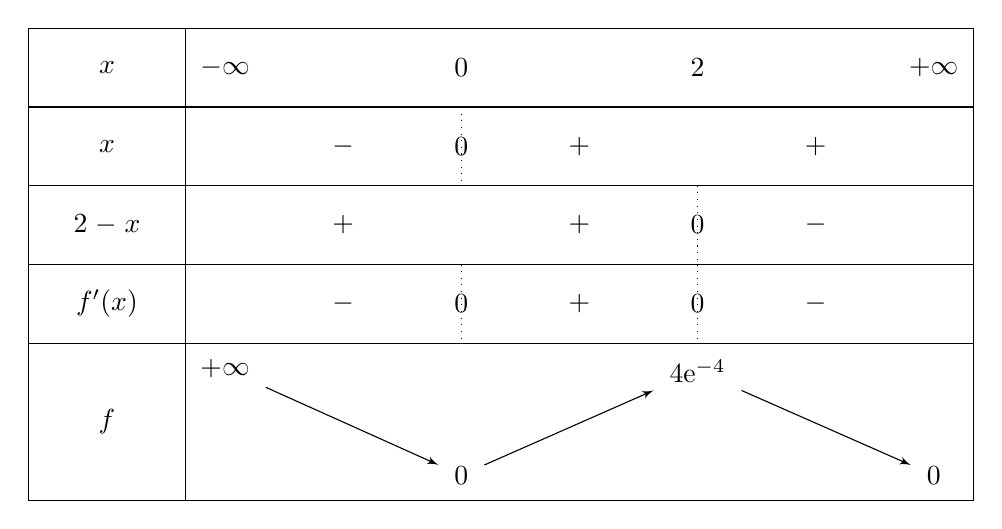
\begin{tikzpicture}[scale=1]
   \tkzTabInit{$x$ / 1 , $x$/1, $2-x$/1, $f'(x)$ / 1, $f$ / 2}{$-\infty$, $0$, $2$, $+\infty$}
   \tkzTabLine{, -, z,+,,+,  }
   \tkzTabLine{, +, ,+,z,-,  }
   \tkzTabLine{, -,z,+,z,-,  }
   \tkzTabVar{+/$+\infty$,-/$0$,+/$4\e^{-4}$, -/$0$}
\end{tikzpicture}
\end{center}

\item  D'après la question précédente, pour tout réel \(x\in [0;4]\), \(0 \leqslant f(x) \leqslant 4\e^{-4}\).

\item On en déduit que \(\displaystyle \int _0^4 0 \dx \leqslant \displaystyle \int _0^4 f(x)\dx \leqslant \displaystyle \int _0^4 4\e^{-4}\dx\) soit  \(0 \leqslant \displaystyle \int _0^4 f(x)\dx \leqslant 16\e^{-4}\).

\item Soit \(g:x\mapsto (ax^2+bx+c)\e^{-x}\). \(g\) est dérivable sur \(\mathbb{R}\) et pour tout réel \(x\), 
	\[g'(x)=(2ax+b)\e^{-x} -(ax^2+bx+c)\e^{-x}=(-ax^2 +(2a-b)x + b-c)\e^{-x}.\]

	Il suffit alors de prendre \(a\), \(b\) et \(c\) de telle sorte que \(-a=1\), \(2a-b=0\) et \(b-c = 0\). Ainsi, \(a=-1\), \(b=-2\) et \(c=-2\) conviennent. Une primitive de \(f\) est donc \(g:x\mapsto -(x^2+2x+2)\e^{-x}\). De fait,
\[\displaystyle \int _0^4 f(x)\dx = \left[-(x^2+2x+2)\e^{-x}\right]_0^4 = 2 -26\e^{-4}.\]


\item Pour tout réel \(x\), on pose \(u(x)=x^2\) et \(v(x)=-\e^{-x}\). On a alors \(u'(x)=2x\) et \(v'(x)=\e^{-x}\). D'après la formule d'intégration par parties, on a
\[ \displaystyle \int _0^4 x^2\e^{-x}\dx = \displaystyle \int _0^4 (uv')(x)\dx = [uv]_0^4 - \displaystyle \int _0^4 (u'v)(x)\dx.\]
	Ainsi, 
\[ \displaystyle \int _0^4 x^2\e^{-x}\dx = \left[-x^2\e^{-x}\right]_0^4 - \displaystyle \int _0^4 2x \times (-\e^{-x})\dx = -16\e^{-4}+2\displaystyle \int _0^4x\e^{-x}\dx.\]

	Pour tout réel \(x\), on pose alors \(w(x) =x\). D'après la formule d'intégration par parties, on a
\[ \displaystyle \int _0^4 x\e^{-x}\dx = \displaystyle \int _0^4 (wv')(x)\dx = [wv]_0^4 - \displaystyle \int _0^4 (w'v)(x)\dx.\]

	et donc 
\[ \displaystyle \int _0^4 x\e^{-x}\dx = \left[-x\e^{-x}\right]_0^4 - \displaystyle \int _0^4 -\e^{-x}\dx = -4\e^{-4} - \left[\e^{-x}\right]_0^4 = 1-5\e^{-4}.\]

	Ainsi, 
\[ \displaystyle \int _0^4 x^2\e^{-x}\dx = -16\e^{-4}+2(1-5\e^{-4})=2-26\e^{-4}.\]
\end{enumerate}
\end{solution}







\begin{exercise}[subtitle={(Sujet zéro 2024)}]

L'exercice est constitué de deux parties indépendantes.

\paragraph{Partie I}

Pour tout entier $n$ supérieur ou égal à 1, on désigne par $f_n$ la fonction définie sur $[0;1]$ par $f_n(x)=x^n\e^x$

On note $C_n$ la courbe représentative de la fonction $f_n$ dans un repère $\Oij$ du plan. On désigne par $I_n$ la suite définie pour tout entier $n$ supérieur ou égal à 1 par $I_n=\displaystyle\int_0^1x^n\e^x\dx$.

\begin{enumerate}
\item \begin{enumerate} 
\item On désigne par $F_1$ la fonction définie sur $[0;1]$ par $F_1(x)=(x-1)\e^x$.\\ Vérifier que $F_1$ est une primitive de la fonction $f_1$.
\item Calculer $I_1$.
\end{enumerate}
\item À l'aide d'une intégration par parties, établir la relation, pour tout entier $n$ supérieur ou égal à 1, \[I_{n+1}=e-(n+1)I_n.\]
\item Calculer $I_2$.
\item On considère la fonction \textbf{mystere} écrite dans le langage Python.

\begin{lstlisting}[language=python]
from math import e #la constante d'Euler e

def mystere(n):
	a = 1
	L = [a]
	for i in range(1,n):
		a = e - (i + 1) * a
		L.append(a)
	return L
\end{lstlisting}

À l'aide des questions précédentes, expliquer ce que renvoie l'appel \textbf{mystere(5)}.

\end{enumerate}
\newpage 
\paragraph{Partie II}

\begin{enumerate}

\item Sur le graphique ci-dessous, on a représenté les courbes $C_1$, $C_2$, $C_3$, $C_{10}$, $C_{20}$ et $C_{30}$.
\begin{center}
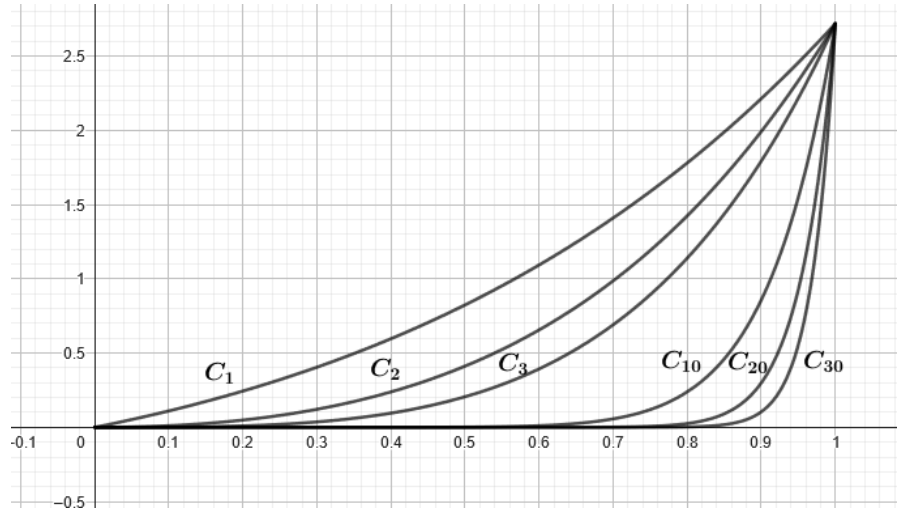
\includegraphics[scale=0.4]{zero2024}
\end{center}
\begin{enumerate}
\item Donner une interprétation graphique de $I_n$.
\item Quelle conjecture peut-on émettre sur la limite de la suite $(I_n)$ ?
\end{enumerate}
\item Montrer que pour tout entier $n$ supérieur ou égal à 1, $0\leqslant I_n \leqslant \e \displaystyle\int_0^1x^n \dx$.
\item En déduire $\displaystyle\lim_{n \to +\infty}I_n$.
\end{enumerate}
\end{exercise}

\begin{solution}
\textbf{Partie I}

\begin{enumerate}
\item \begin{enumerate}
\item Pour tout réel $x\in [0;1]$, $F_1'(x)=1 \times \e^x+(x-1)\times\e^x=x\e^x$. $F_1$ est bien une primitive de $f_1$ sur $[0;1]$.
\item On a $I_1=\displaystyle\int_0^1f_1(x)\dx=[F_1(x)]_0^1=F_1(1)-F_1(0)=0-(-1)=1$.
\end{enumerate}
\item On a $I_{n+1}=\displaystyle\int_0^1x^{n+1}\e^x\dx$.
Pour tout réel $x\in [0;1]$, on pose $u(x)=x^{n+1}$ et $v(x)=\e^x$.\\ On a alors $u'(x)=(n+1)x^n$ et $v'(x)=\e^x$. Ainsi, d'après la formule d'intégration par parties,
\[I_{n+1}=\displaystyle\int_0^1 uv'(x)\dx = [uv(x)]_0^1-\displaystyle\int_0^1u'v(x)\dx=[x^{n+1}\e^x]_0^1-\displaystyle\int_0^1 (n+1)x^n\e^x\dx=e-(n+1)I_{n}.\]
\item On a $I_2=I_{1+1}=e-(1+1)I_1=e-2$.
\item L'appel \textbf{mystere(5)} renvoie la liste des 5 premières valeurs de la suite $(I_n)$.
\end{enumerate}

\textbf{Partie II}

\begin{enumerate}
\item \begin{enumerate}
\item $(I_n)$ représente l'aire délimité par la courbe $C_n$, l'axe des abscisses et les droites d'équation $x=0$ et $x=1$.
\item Il semblerait que l'aire sous la courbe se rapproche de 0, soit $\displaystyle\lim_{n \to +\infty}I_n=0$.
\end{enumerate}
\item D'une part, pour tout réel $x\in[0;1]$, on a $f_n(x)\geqslant 0$. Par ailleurs, la fonction exponentielle étant croissante, alors pour tout $x\in[0;1]$, $\e^x \leqslant \e^1$ et donc $f_n(x)\leqslant \e x^n$. En intégrant, on a donc bien $0 \leqslant I_n \leqslant \e \displaystyle\int_0^1x^n \dx$.
\item On a $\e \displaystyle\int_0^1x^n \dx=\e \times \left[\dfrac{x^{n+1}}{n+1}\right]_0^1=\dfrac{\e}{n+1}$. Or, $\displaystyle\lim_{n \to +\infty}\dfrac{\e}{n+1}=0$. Par ailleurs, $\displaystyle\lim_{n \to + \infty}0=0$. Or, on a vu que pour tout entier naturel non nul $n$, on a $0 \leqslant I_n \leqslant \e \displaystyle\int_0^1x^n \dx$. D'après le théorème d'encadrement, on a donc $\displaystyle\lim_{n \to +\infty}I_n=0$.
\end{enumerate}

\end{solution}


\begin{exercise}[subtitle={(Métropole 2024)}]

\paragraph{Partie A : étude de la fonction $f$}

La fonction $f$ est définie sur l'intervalle $]0;+\infty[$ par $f(x)=x-2+\dfrac{1}{2}\ln (x)$, où $\ln$ désigne la fonction logarithme népérien. On admet que la fonction $f$ est deux fois dérivables sur $]0;+\infty[$, on note $f'$ sa dérivée et $f''$ sa dérivée seconde.

\begin{enumerate}
\item \begin{enumerate}
\item Déterminer, en justifiant, les limites de $f$ en 0 et en $+\infty$.
\item Montrer que pour tout $x$ appartenant à $]0;+\infty [$, on a $f'(x)=\dfrac{2x+1}{2x}$.
\item Étudier le sens de variations de $f$ sur $]0;+\infty[$.
\item Étudier la convexité de $f$ sur $]0 ;+\infty[$.
\end{enumerate}
\item \begin{enumerate}
\item Montrer que l'équation $f(x)=0$ admet dans $]0;+\infty[$ une solution unique qu'on notera $\alpha$ et justifier que $\alpha$ appartient à l'intervalle $[1;2]$.
\item Déterminer le signe de $f(x)$ pour $x\in ]0;+\infty[$.
\item Montrer que $\ln(\alpha)=2(2-\alpha)$.
\end{enumerate}\end{enumerate}

\paragraph{Partie B : étude de la fonction $g$}

La fonction $g$ est définie sur $]0;1]$ par $g(x)=-\dfrac{7}{8}x^2+x-\dfrac{1}{4}x^2\ln(x)$. On admet que la fonction $g$ est dérivable sur $]0;1]$ et on note $g'$ sa fonctione dérivée.

\begin{enumerate}
\item Calculer $g'(x)$ pour $x\in ]0;1]$ puis vérifier que $g'(x)=xf\left(\dfrac{1}{x}\right)$.
\item \begin{enumerate}
\item Justifier que pour $x$ appartenant à l'intervalle $ \left] 0 ; \dfrac{1}{\alpha} \right[$, on a $f\left(\dfrac{1}{x}\right)>0$.
\item On admet le tableau de signes suivant :

\begin{center}
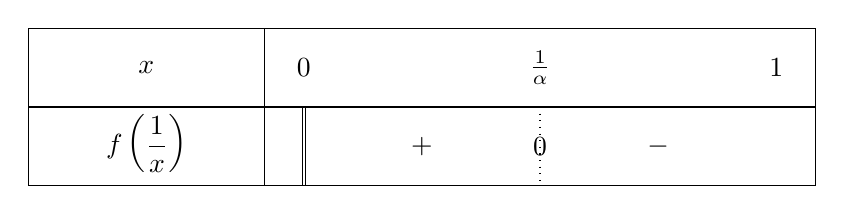
\begin{tikzpicture}[scale=1]
\tikzset{node style/.style = {inner sep = 2pt, outer sep = 2pt}}
   \tkzTabInit[lgt=3]{$x$ / 1, $f\left(\dfrac{1}{x}\right)$ / 1}{$0$, $\frac{1}{\alpha}$, $1$}
   \tkzTabLine{d,+,z, -,  }
\end{tikzpicture}\end{center}

En déduire le tableau de variations de $g$ sur l'intervalle $]0;1]$. Les images et les limites ne sont pas demandées.
\end{enumerate}
\end{enumerate}


\paragraph{Partie C : un calcul d'aire}

On a représenté sur le graphique ci-dessous
\begin{itemize}
\item La courbe $\mathcal{C}_g$ de la fonction $g$ ;
\item La parabole $\mathcal{P}$ d'équation $y=-\dfrac{7}{8}x^2+x$ sur l'intervalle $]0;1]$.
\end{itemize}

\begin{center}
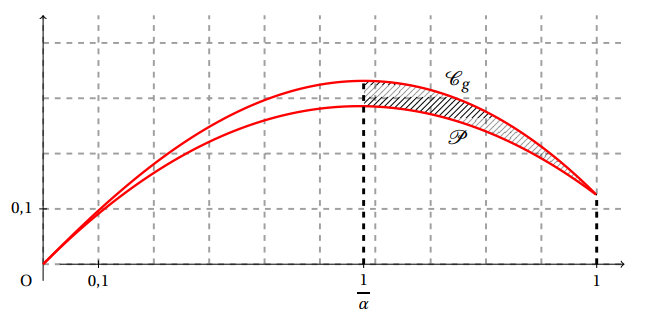
\includegraphics[scale=0.5]{metro2024}
\end{center}

On souhaite calculer l'aire $\mathcal{A}$ du domaine hachuré compris entre les courbes $\mathcal{C}_g$, $\mathcal{P}$ et les droites d'équation $x=\dfrac{1}{\alpha}$ et $x=1$.

On rappelle que $\ln(\alpha)=2(2-\alpha)$.

\begin{enumerate}
\item \begin{enumerate}
\item Justifier la position relative des courbes $\mathcal{C}_g$ et $\mathcal{P}$ sur l'intervalle $]0;1]$.
\item Démontrer l'égalité
\[\displaystyle\int_{\frac{1}{\alpha}}^1 x^2 \ln(x) \dx = \dfrac{-\alpha ^3 -6\alpha +13}{9\alpha ^3}\]
\end{enumerate}
\item En déduire l'expression en fonction de $\alpha$ de l'aire $\mathcal{A}$.
\end{enumerate}

\end{exercise}

\begin{solution}

\textbf{Partie A : étude de la fonction $f$}

\begin{enumerate}
\item \begin{enumerate}
\item On a $\displaystyle\lim_{x \to 0}(x-2)=-2$ et $\displaystyle\lim_{x\to 0^+}\ln(x)=-\infty$. Par somme, $\displaystyle\lim_{x\to 0}f(x)=-\infty$.

Par ailleurs, $\displaystyle\lim_{x\to +\infty}(x-2)=+\infty$ et $\displaystyle\lim_{x\to +\infty}\ln(x)=+\infty$. Par somme, on a $\displaystyle\lim_{x\to +\infty}f(x)=+\infty$.
\item Pour tout $x>0$, on a $f'(x)=1+\dfrac{1}{2} \times \dfrac{1}{x}=\dfrac{2x}{2x}+\dfrac{1}{2x}=\dfrac{2x+1}{x}$.
\item Puisque pour tout $x>0$, on a $2x+1>0$, la fonction $f$ est strictement croissante sur $]0;+\infty[$. (on aurait également pu dire que la somme de deux fonctions croissantes est croissante...).
\item Pour tout réel $x>0$, $f''(x)=\dfrac{2 \times 2x - (2x+1) \times 2}{(2x)^2}=-\dfrac{2}{(2x)^2}<0$.\\ La fonction $f$ est concave sur $]0;+\infty[$.
\end{enumerate}
\item \begin{enumerate}
\item La fonction $f$ est continue sur $]0;+\infty[$. De plus, $\displaystyle\lim_{x \to 0}f(x)=-\infty$ et $\displaystyle\lim_{x\to +\infty}f(x)=+\infty$. D'après le théorème des valeurs intermédiaires, l'équation $f(x)=0$ admet une solution sur l'intervalle $]0;+\infty[$. De plus, la fonction $f$ étant strictement croissante sur cet intervalle, cette solution est unique.

En outre, on a $f(1)=-1$ et $f(2)=\dfrac{1}{2}\ln(2)>0$. On peut donc affirmer que $\alpha \in [1;2]$.

\item On a le tableau de signes suivant.

\begin{center}
	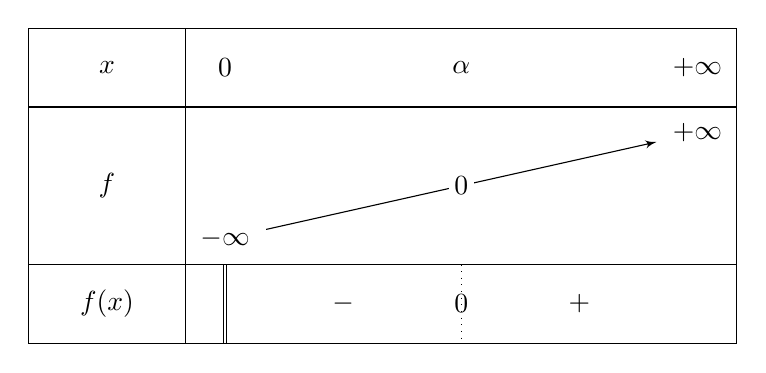
\begin{tikzpicture}[scale=1]
   \tkzTabInit{$x$ / 1 , $f$/ 2, $f(x)$ / 1}{$0$, $\alpha$, $+\infty$}

   \tkzTabVar{-/$-\infty$,R/,+/$+\infty$}
   \tkzTabIma{1}{3}{2}{$0$}
      \tkzTabLine{d,-, z,+,  }
\end{tikzpicture}
\end{center}

\end{enumerate}

\item On sait que $f(\alpha)=0$, c'est-à-dire $\alpha-2+\dfrac{1}{2}\ln(\alpha)=0$. Ainsi, $\dfrac{1}{2}\ln(\alpha)=2-\alpha$ et donc $\ln(\alpha)=2(2-\alpha)$.

\end{enumerate}

\textbf{Partie B : étude de la fonction $g$}

\begin{enumerate}
\item Pour tout réel $x\in ]0;1]$, on a \[g'(x)=-\dfrac{7}{8} \times 2x + 1 - \dfrac{1}{4}\left(2x \times \ln(x) +x^2 \times \dfrac{1}{x}\right)=-\dfrac{7}{4}x+1-\dfrac{1}{2}x\ln(x)-\dfrac{1}{4}x=-2x+1-\dfrac{1}{2}x\ln(x).\]
Ainsi, \[g'(x)=x\left(\dfrac{1}{x}-2-\dfrac{1}{2}\ln(x)\right)=x\left(\dfrac{1}{x}-2+\dfrac{1}{2}\ln\left(\dfrac{1}{x}\right)\right)=xf\left(\dfrac{1}{x}\right).\]
\item \begin{enumerate}
\item Soit $x\in \left]0;\dfrac{1}{\alpha}\right[$, on a alors $0<x< \dfrac{1}{\alpha}$ et donc $\dfrac{1}{x}>\alpha$. Puisque la fonction $f$ est strictement croissante sur $]0;+\infty[$, on a alors $f\left(\dfrac{1}{x}\right)>f(\alpha)$. Or, $f(\alpha)=0$. Ainsi, $f\left(\dfrac{1}{x}\right)>0$.
\item On sait que pour tout $x\in]0;1]$, $g'(x)$ est du signe de $f\left(\dfrac{1}{x}\right)$. On en déduit le tableau de variations de $g$.

\begin{center}
	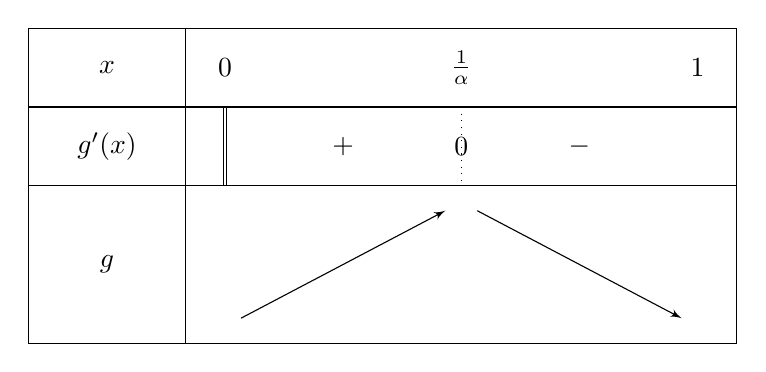
\begin{tikzpicture}[scale=1]
   \tkzTabInit{$x$ / 1 , $g'(x)$/ 1, $g$ / 2}{$0$, $\frac{1}{\alpha}$, $1$}
      \tkzTabLine{d,+, z,-,  }
   \tkzTabVar{-/$ $, +/$ $,-/$ $}

\end{tikzpicture}
\end{center}

\end{enumerate}
\end{enumerate}


\textbf{Partie C : un calcul d'aire}

\begin{enumerate}
\item \begin{enumerate}
\item Pour tout réel $x\in]0;1]$, on note $h(x)=-\dfrac{7}{8}x^2+x$. On a alors
\[g(x)-h(x)=-\dfrac{7}{8}x^2+x-\dfrac{1}{4}x^2\ln(x)-\left(-\dfrac{7}{8}x^2+x\right)=-\dfrac{1}{4}x^2\ln(x).\]
Or, pour tout $x\in]0;1]$, $x^2>0$. De plus, la fonction logarithme népérien étant croissante sur $]0;1]$, on a alors $\ln(x)\leqslant \ln(1)$ soit $\ln(x)\leqslant 0$. Ainsi, pour tout $x\in ]0;1]$, $g(x)-h(x)\geqslant 0$. La courbe $\mathcal{C}_g$ est donc au-dessus de $\mathcal{P}$.
\item On souhaite calculer $\displaystyle\int_{\frac{1}{\alpha}}^1 x^2 \ln(x) \dx$. Pour tout réel $x\in \left[\dfrac{1}{\alpha} ; 1 \right]$, on pose $u(x)=\ln(x)$ et $v(x)=\dfrac{x^3}{3}$. On a alors $u'(x)=\dfrac{1}{x}$ et $v'(x)=x^2$. D'après la formule d'intégration par parties, 
\[\displaystyle\int_{\frac{1}{\alpha}}^1 x^2 \ln(x) \dx = \left[ \dfrac{x^3\ln(x)}{3}\right]_{\frac{1}{\alpha}}^1-\displaystyle\int_{\frac{1}{\alpha}}^1 \dfrac{x^3}{3} \times \dfrac{1}{x}\dx=0-\dfrac{\ln\left(\frac{1}{\alpha}\right)}{3\alpha ^3}-\displaystyle\int_{\frac{1}{\alpha}}^1 \dfrac{x^2}{3}\dx = \dfrac{\ln\left(\alpha\right)}{3\alpha ^3}-\left[\dfrac{x^3}{9}\right]_{\frac{1}{\alpha}}^1=\dfrac{\ln\left(\alpha\right)}{3\alpha ^3} - \left( \dfrac{1}{9} - \dfrac{1}{9\alpha ^3}\right).\]
On a utilisé le fait que $\ln\left(\dfrac{1}{\alpha}\right)=-\ln(\alpha)$. On rappelle alors que $\ln(\alpha)=2(2-\alpha)$. Ainsi,
\[\displaystyle\int_{\frac{1}{\alpha}}^1 x^2 \ln(x) \dx=\dfrac{2(2-\alpha)}{3\alpha ^3}-\dfrac{1}{9}+\dfrac{1}{9 \alpha ^3}=\dfrac{12-6\alpha}{9\alpha^3}-\dfrac{\alpha ^3}{9\alpha^3}+\dfrac{1}{9 \alpha^3} = \dfrac{-\alpha ^3 + 6\alpha + 13}{9\alpha ^3}.\]
\end{enumerate}
\item L'aire hachurée vaut \[\mathcal{A}=\int_{\frac{1}{\alpha}}^1(g(x)-h(x))\dx=\int_{\frac{1}{\alpha}}^1\left(-\dfrac{1}{4}x^2\ln(x)\right)\dx=-\dfrac{1}{4} \times \dfrac{-\alpha^3-6\alpha+13}{9\alpha ^3}.\]
\end{enumerate}


\end{solution}


\begin{exercise}Pour tout $n \in\mathbb{N}$, on pose $I_n=\displaystyle\int_0^1x^n \ln(1+x)\dx$.
\begin{enumerate}
\item Calculer $I_0$.
\item Montrer que la suite $(I_n)$ est positive et décroissante. Que peut-on en déduire ?
\item \begin{enumerate}
\item Montrer que, pour tout entier naturel $n$ et tout $x\in [0;1]$, $x^n \ln(1+x) \leqslant x^n$.
\item En déduire que pour tout $n \in \mathbb{N}$, $I_n \leqslant \dfrac{1}{n+1}$.
\item En déduire $\displaystyle\lim_{n \to+\infty}I_n$.
\end{enumerate}
\item \begin{enumerate}
\item En effectuant une intégration par partie, montrer que pour tout entier naturel $n$, on a
\[I_n = \dfrac{\ln(2)}{n+1}-\dfrac{1}{n+1}\int_0^1\dfrac{x^{n+1}}{1+x}\dx.\]
\item Étudier la convergence de la suite $(nI_n)$.
\end{enumerate}
\end{enumerate}\end{exercise}

\begin{solution}\hspace{0pt}

	\begin{enumerate}
\item  On a \(I_0=\displaystyle\int_0^1\ln(1+x)\dx\). On procède à une intégration par parties, en posant, pour tout réel \(x\) entre 0 et 1, \(u(x)=x\) (et donc \(u'(x)=1\)) et \(v(x)=\ln(1+x)\). Ainsi,
\[\displaystyle\int_0^1\ln(1+x)\dx = \left[x\ln(1+x)\right]_0^1-\displaystyle\int_0^1 \dfrac{x}{1+x}\dx.\]
D'une part, \(\left[x\ln(1+x)\right]_0^1=\ln(2)\). Par ailleurs, pour tout réel \(x \in [0;1]\), \(\dfrac{x}{1+x}=1-\dfrac{1}{1+x}\). Ainsi, 
\[\displaystyle\int_0^1\ln(1+x)\dx = \ln (2)- \left[x-\ln(1+x)\right]_0^1 = \ln(2)-(1-\ln(2))=2\ln(2)-1.\]

\item  Pour tout entier naturel \(n\), pour tout réel \(x \in [0;1]\) on a \(0 \leqslant x^{n+1}\leqslant x^n\). Par ailleurs, pour tout réel \(x\in[0;1]\), \(1+x \geqslant 1\) et donc, en appliquant la fonction logarithme népérien qui est croissante sur \([1;+\infty[\), on a donc que \(\ln(1+x)\geqslant 0\).
	Finalement, pour tout entier naturel \(n\), pour tout réel \(x \in [0;1]\), \(0 \leqslant x^{n+1}\ln(1+x) \leqslant x^n\ln(1+x)\). En intégrant cette inégalité entre 0 et 1, on a donc que, pour tout entier naturel \(n\), \(0 \leqslant I_{n+1} \leqslant I_n\). La suite \((I_n)\) est positive et décroissante, elle est donc convergente.
\item  \begin{enumerate}
\item  Pour tout \(x\in [0,1]\), \(1 \leqslant 1+x \leqslant 2\) et donc \(0 \leqslant\ln(1+x)\leqslant \ln(2)\), qui est lui-même inférieur à 1. Ainsi, pour tout entier naturel \(n\) et tout \(x\in [0;1]\), \(x^n \ln(1+x) \leqslant x^n\).
\item  En intégrant cette dernière inégalité entre 0 et 1, on en déduit que pour tout \(n \in \mathbb{N}\), \(I_n \leqslant \displaystyle\int_0^1x^n\dx\). Or, \[\displaystyle\int_0^1 x^n \dx=\left[\dfrac{x^{n+1}}{n+1}\right]_0^1=\dfrac{1}{n+1}.\]
Ainsi, pour tout entier naturel \(n\), \(I_n \leqslant \dfrac{1}{n+1}\).
\item  On sait que pour tout entier naturel \(n\), \(0 \leqslant I_n \leqslant \dfrac{1}{n+1}\). Or, \(\displaystyle\lim_{n \to + \infty}0 = \displaystyle\lim_{n \to + \infty}\dfrac{1}{n+1}=0\). D'après le théorème d'encadrement, la suite \((I_n)\) converge (ce que l'on avait déjà démontré) et \(\displaystyle\lim_{n \to+\infty}I_n=0\).
\end{enumerate}
\item  \begin{enumerate}
\item  Soit \(n\) un entier naturel. Pour tout \(x\in [0;1]\), on pose \(u(x)=\ln(1+x)\) et \(v(x)=\dfrac{x^{n+1}}{n+1}\) (on a alors \(v'(x)=x^n\)). Par intégration par parties, on a alors
\[I_n = \left[\dfrac{x^{n+1}\ln(1+x)}{n+1}\right]_0^1-\dfrac{1}{n+1}\int_0^1\dfrac{x^{n+1}}{1+x}\dx = \dfrac{\ln(2)}{n+1}-\dfrac{1}{n+1}\int_0^1\dfrac{x^{n+1}}{1+x}\dx .\]
\item  Pour tout entier naturel \(n\),
\[nI_n = \dfrac{n\ln(2)}{n+1}-\dfrac{n}{n+1}\int_0^1\dfrac{x^{n+1}}{1+x}\dx .\] 
Or, \(\displaystyle\lim_{n \to + \infty}\dfrac{n}{n+1}=1\) (on peut factoriser par \(n\) ou écrire \(\dfrac{n}{n+1}=1-\dfrac{1}{n+1}\)). Par ailleurs, pour tout réel \(x\in [0;1]\), \(\dfrac{x^n}{2} \leqslant \dfrac{x^{n+1}}{1+x} \leqslant x^n\) et donc, en intégrant entre 0 et 1,
\[ \dfrac{1}{2(n+1)} \leqslant \int_0^1\dfrac{x^{n+1}}{1+x}\dx \leqslant \dfrac{1}{n+1}.\]
Ainsi, en utilisant le théorème d'encadrement, on trouve que cette intégrale converge et que \[\displaystyle\lim_{n \to + \infty}\int_0^1\dfrac{x^{n+1}}{1+x}\dx =0\] Finalement, la suite \((nI_n)\) converge et \(\displaystyle\lim_{n \to + \infty} nI_n=\ln(2)\).

\end{enumerate}\end{enumerate}

\end{solution}





\chapter{Corrigés}


\printsolutions[headings={false} ]

\end{document}